\documentclass[xcolor={dvipsnames}, aspectratio=169]{beamer}
\usepackage{beamerthemesplit}
\usepackage{wrapfig}
\usetheme{SPbGU}
\usepackage{pdfpages}
\usepackage{amsmath}
\usepackage{amssymb}
\usepackage{cmap}
\usepackage[T2A]{fontenc}
\usepackage[utf8]{inputenc}
\usepackage[english]{babel}
\usepackage{indentfirst}
\usepackage[absolute,overlay]{textpos}
\usepackage{tikz}
\usetikzlibrary{shapes,arrows,arrows.meta,automata,positioning,quotes,backgrounds,decorations.text,decorations.pathmorphing}
\usepackage{multirow}
\usepackage[noend]{algpseudocode}
\usepackage{algorithm}
\usepackage{algorithmicx}
\usepackage{fancyvrb}
\usepackage[linguistics]{forest}
\usepackage{listings}
\usepackage{multicol}
\usepackage{comment}
\usepackage{xspace}
\usepackage{adjustbox}
\usepackage{makecell}
\usepackage{ stmaryrd }
\usepackage{ulem}
\usepackage{wasysym}
\usepackage{amssymb}
\usepackage{pifont}
\usepackage{animate}
\definecolor{ForestGreen}{RGB}{34,139,34}

\usepackage{amsmath}
\usepackage{xspace}
\usepackage{listings}
\usepackage{subcaption}
\usepackage{multirow}
\usepackage{multicol}
\usepackage{balance}
\usepackage{microtype}
\usepackage{siunitx}
\usepackage{iftex}
\usepackage{indentfirst}


\newcommand{\cmark}{\textcolor{green}{\ding{51}}}
\newcommand{\xmark}{\textcolor{red}{\ding{55}}}

\newcommand{\todelete}[1]{{\color{red}{#1}}}

\newcommand{\subdued}[1]{{\color{gray}{#1}}}

\newcommand{\backupbegin}{
   \newcounter{finalframe}
   \setcounter{finalframe}{\value{framenumber}}
}
\newcommand{\backupend}{
   \setcounter{framenumber}{\value{finalframe}}
}

\newcommand{\happyCheck}{\color{green}{\checkmark}}
\newcommand{\timeout}{\color{red}{\clock}}

\newcommand{\makenote}[1]{\hfill \footnotesize{#1}}
\newcommand{\strikeoutnote}[1]{\makenote{\strikethrough{#1}}}
\newcommand{\strikethrough}[1]{\sout{#1}}

\newcommand{\lststrikethrough}[1]{\ttfamily\sout{#1}}

\newcolumntype{A}{>{\hb@xt@\z@\bgroup\hss}r<{\egroup}}
\newcolumntype{B}{>{\hb@xt@\z@\bgroup}l<{\hss\egroup}}

\setbeamertemplate{itemize item}[circle]
\setbeamertemplate{enumerate items}[circle]

\lstdefinelanguage{ocanren1}{
  basicstyle = {\ttfamily \color{black}},
  keywords=[1]{return, do, where, case, run, conde, fresh, let, match, with, when, class,
  object, method, of, rec, repeat, until, while, \begin{comment}not,\end{comment} do, done, as, val, inherit,
  new, module, sig, deriving, datatype, struct, if, then, else, open, private, virtual, include, success, failure,
  true, false, mplus},
  keywords=[2]{safe},
  keywords=[3]{unsafe},
  sensitive=true,
  commentstyle=\small\itshape\ttfamily,
  keywordstyle=[1]\color{blue},
  keywordstyle=[2]\color{ForestGreen},
  keywordstyle=[3]\color{violet},
  identifierstyle=\ttfamily,
  basewidth={0.5em,0.5em},
  columns=flexible,
  mathescape=true,
  escapechar=~,
  fontadjust=true,
  literate={fun}{{$\lambda$}}1 {function}{function}8 {->}{{$\to$}}3 {<-}{{$\leftarrow$}}3 {===}{{$\equiv$}}1 {=/=}{{$\not\equiv$}}1 {|>}{{$\triangleright$}}3 {\\/}{{$\vee$}}2 {/\\}{{$\wedge$}}2 {^}{{$\uparrow$}}1,
  morecomment=[s]{(*}{*)},
  moredelim=**[is][\color{red}]{@!}{@}
}

\lstdefinelanguage{ocanren}{
  basicstyle = {\ttfamily \color{black} \footnotesize},
  keywords=[1]{return, do, where, case, run, conde, fresh, let, match, with, when, class,
  object, method, of, rec, repeat, until, while, \begin{comment}not,\end{comment} do, done, as, val, inherit,
  new, module, sig, deriving, datatype, struct, if, then, else, open, private, virtual, include, success, failure,
  true, false, mplus, data, instance},
  backgroundcolor = {\color{Orchid!10}},
  keywords=[2]{safe},
  keywords=[3]{unsafe},
  sensitive=true,
  commentstyle=\small\itshape\ttfamily,
  keywordstyle=[1]\color{blue},
  keywordstyle=[2]\color{ForestGreen},
  keywordstyle=[3]\color{violet},
  identifierstyle=\ttfamily,
  basewidth={0.5em,0.5em},
  columns=flexible,
  mathescape=true,
  escapechar=~,
  fontadjust=true,
  literate={fun}{{$\lambda$}}1 {function}{function}8 {->}{{$\to$}}3 {<-}{{$\leftarrow$}}3 {===}{{$\equiv$}}1 {=/=}{{$\not\equiv$}}1 {\\/}{{$\vee$}}2 {/\\}{{$\wedge$}}2 {^}{{$\uparrow$}}1,
  morecomment=[s]{(*}{*)},
  moredelim=**[is][\color{red}]{@!}{@}
}

% \lstset{
%   language=ocanren
% }


\lstdefinelanguage{imperative}{
  basicstyle = {\ttfamily \color{black} \tiny},
  backgroundcolor = {\color{ForestGreen!10}},
  keywordstyle = {\color{blue}},
  keywordstyle = [2]{\color{ForestGreen}},
  keywords = {while, do, if, then, return, procedure, for, fun, else}, 
  morekeywords = [2]{true, false, none},
}

\lstdefinelanguage{racket}{
  basicstyle = {\ttfamily \color{black} \footnotesize},
  backgroundcolor = {\color{Emerald!10}},
  keywordstyle = {\color{blue}},
  keywordstyle = [2]{\color{ForestGreen}},
  keywords = {while, do, if, then, return, procedure}, 
  morekeywords = [2]{true, false, none},
}

\lstdefinelanguage{logic}{
  basicstyle = {\ttfamily \color{black} \footnotesize},
  backgroundcolor = {\color{SkyBlue!10}},
  keywordstyle = {\color{blue}},
  keywordstyle = [2]{\color{ForestGreen}},
  keywords = {while, do, if, then, return, procedure}, 
  morekeywords = [2]{start, end},
}

\lstdefinelanguage{query}{
  basicstyle = {\ttfamily \color{black}},
  backgroundcolor = {\color{Periwinkle!10}},
  keywordstyle = {\color{blue}},
  keywordstyle = [2]{\color{ForestGreen}},
  keywords = {true, false}, 
  otherkeywords={<-,->},
  morekeywords = [2]{<-, ->, nondeterminism, predicate,ignore},
}


\lstdefinestyle{mystyle}
{
    language = C++,
    basicstyle = {\ttfamily \color{black}},
    backgroundcolor = {\color{white}},
    stringstyle = {\color{blue}},
    keywordstyle = {\color{green}},
    keywordstyle = [2]{\color{lime}},
    keywordstyle = [3]{\color{yellow}},
    keywordstyle = [4]{\color{teal}},
    otherkeywords = {;,<<,>>,++},
    morekeywords = [2]{true, false},
    morekeywords = [3]{<<, >>},
    morekeywords = [4]{++},
}

\tikzstyle{processTree} = [
  ->,
  sibling distance=15em,
  scale=0.6,
  every node/.style = {
    shape=rectangle,
    rounded corners=0.05cm,
    draw,
    align=center,
    minimum size=5mm,
    scale=0.6,},
  %level 1/.style={sibling distance=100em}
  ]


\tikzstyle{program} = [
  draw=black,
  thick,
  rectangle,
  rounded corners=1pt,
  inner sep=5pt,
  inner ysep=5pt
  ]

\tikzstyle{goal} = [
  draw=black,
  rectangle,
  rounded corners=1pt,
  inner ysep=0pt,
  ]

\tikzstyle{input} = [
  draw=none,
  rectangle,
  rounded corners=1pt,
  inner sep=2pt,
  inner ysep=2pt,
  fill=green!10,
  minimum height=5mm
  ]


\tikzstyle{transparent} = [
  draw=none,
  inner ysep=3pt
  ]



\DeclareMathOperator{\Term}{\mathcal{T}}
\DeclareMathOperator{\FlatTerm}{\mathcal{FT}}
\DeclareMathOperator{\Var}{\mathbf{Var}}
\DeclareMathOperator{\Cons}{\mathcal{C}}
\DeclareMathOperator{\Kan}{\mathcal{G}}
\DeclareMathOperator{\Fresh}{\mathbf{Fresh}}
\DeclareMathOperator{\Delay}{\mathbf{Delay}}
\DeclareMathOperator{\Cll}{\mathbf{Call}}
\DeclareMathOperator{\Def}{\mathcal{D}}
\DeclareMathOperator{\Base}{\mathbf{Base}}
\DeclareMathOperator{\Conj}{\mathbf{Conj}}
\DeclareMathOperator{\free}{\mathbf{free}}
\DeclareMathOperator{\ground}{\mathbf{ground}}
\DeclareMathOperator{\In}{\mathbf{In}}
\DeclareMathOperator{\Out}{\mathbf{Out}}
\DeclareMathOperator{\Fun}{\mathcal{F}}
\DeclareMathOperator{\Rtrn}{\mathbf{return}}
\DeclareMathOperator{\Bind}{\mathbf{Bind}}
\DeclareMathOperator{\Match}{\mathbf{Match}}
\DeclareMathOperator{\Sum}{\mathbf{<|>}}
\DeclareMathOperator{\Guard}{\mathbf{Guard}}
\DeclareMathOperator{\Gen}{\mathbf{Gen}}
\DeclareMathOperator{\Stream}{\mathit{Stream}}
\DeclareMathOperator{\vars}{vars}
\DeclareMathOperator{\inmode}{\mathtt{I}}
\DeclareMathOperator{\outmode}{\mathtt{O}}
\DeclareMathOperator{\whatmode}{\mathtt{?}}
% \DeclareMathOperator{\inmode}{g \rightarrow g}
% \DeclareMathOperator{\outmode}{f \rightarrow g}
% \DeclareMathOperator{\mode1}{mode}
% \DeclareMathOperator{\Mode1}{\mathcal{M}}
\newcommand{\KanN}{\mathcal{K}^{N}}
\newcommand{\tran}[1]{\left\llbracket #1 \right\rrbracket}
\newcommand{\LIST}[1]{ #1^*}
\renewcommand{\emptyset}{\varnothing}
\newcommand{\mk}{\textsc{miniKanren}\xspace}
\newcommand{\ocaml}{\textsc{OCaml}\xspace}
\newcommand{\haskell}{\textsc{Haskell}\xspace}
\renewcommand{\and}{$\&$\xspace}
\newcommand{\rel}[2]{\texttt{#1}$^o$ #2}
\newcommand{\subst}[1]{$\langle$#1$\rangle$}
\newcommand{\sem}[1]{\llbracket #1 \rrbracket}

\lstset{moredelim=[is][\bfseries]{[*}{*]}}

\beamertemplatenavigationsymbolsempty

\title[Typed Embedding of miniKanren]{Typed Embedding of miniKanren for Functional Conversion}
\institute[]{
JetBrains Research, \\
Constructor University, Bremen
}

\author[Ekaterina Verbitskaia]{Igor Engel, \textbf{Ekaterina Verbitskaia}}

\date{October 17, 2025}

\definecolor{orange}{RGB}{179,36,31}

\begin{document}
{

\begin{frame}[fragile]
   \begin{center}
      
\includegraphics[height=1cm]{pictures/jetbrains.pdf}
    \end{center}
  \titlepage
\end{frame}
}

\begin{frame}[fragile]
  \frametitle{No \mk~--- One Task, One Program}
  \begin{columns}    
    \begin{column}{0.35\textwidth}
      \centering
      \vspace{2cm}
      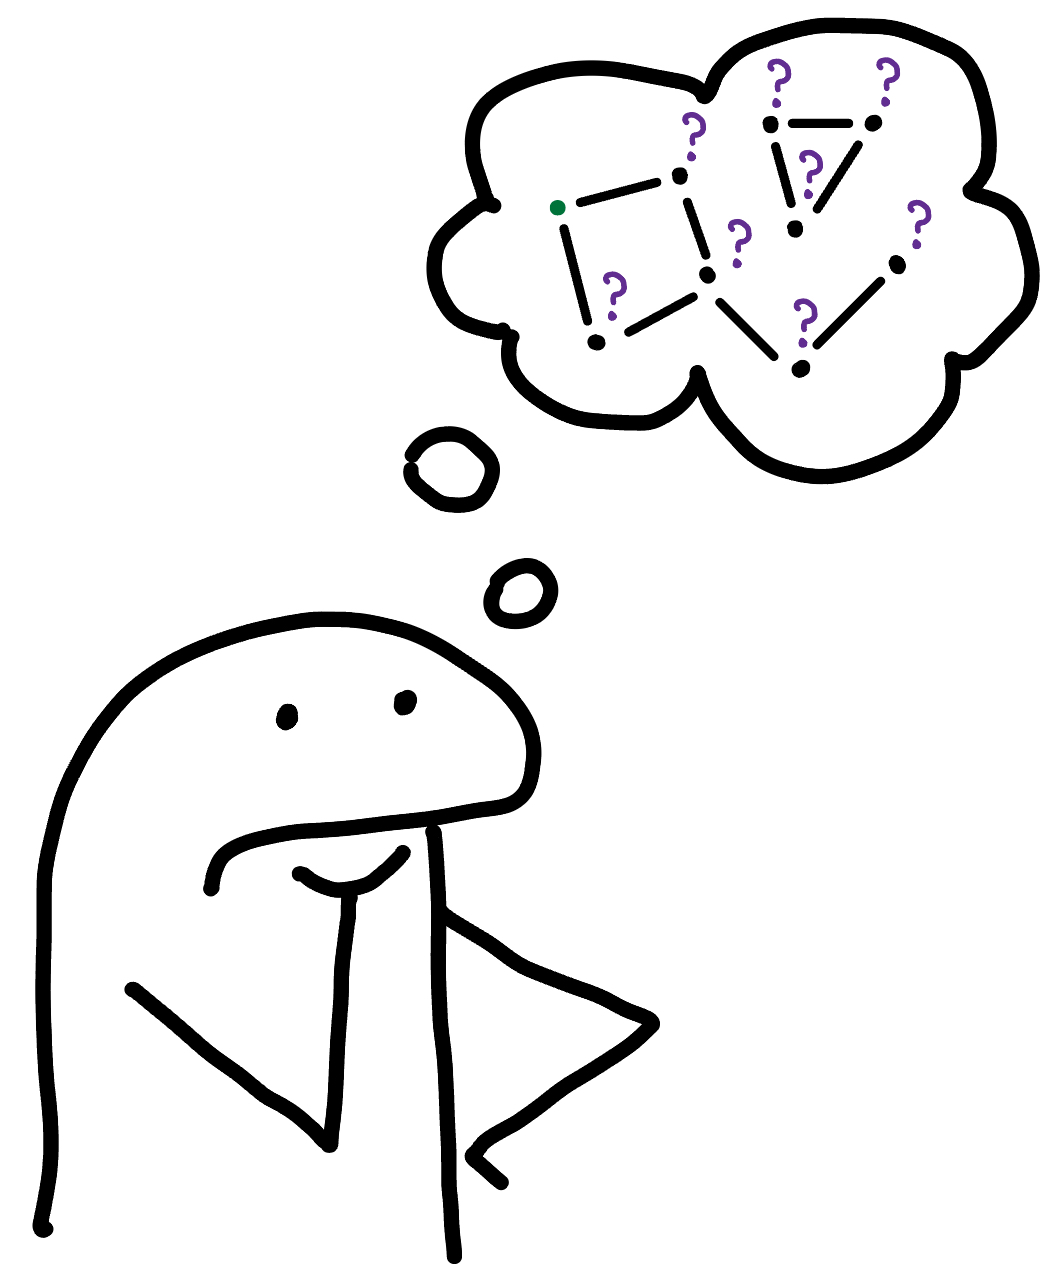
\includegraphics[width=0.8\textwidth]{pic/reachable.jpg}
    \end{column}
    \begin{column}{0.35\textwidth}
    \end{column}
    \begin{column}{0.35\textwidth}
    \end{column} 
  \end{columns}
\end{frame}
\addtocounter{framenumber}{-1}

\begin{frame}[fragile]
  \frametitle{No \mk~--- One Task, One Program}
  \begin{columns}    
    \begin{column}{0.35\textwidth}
      \centering
      \vspace{2cm}
      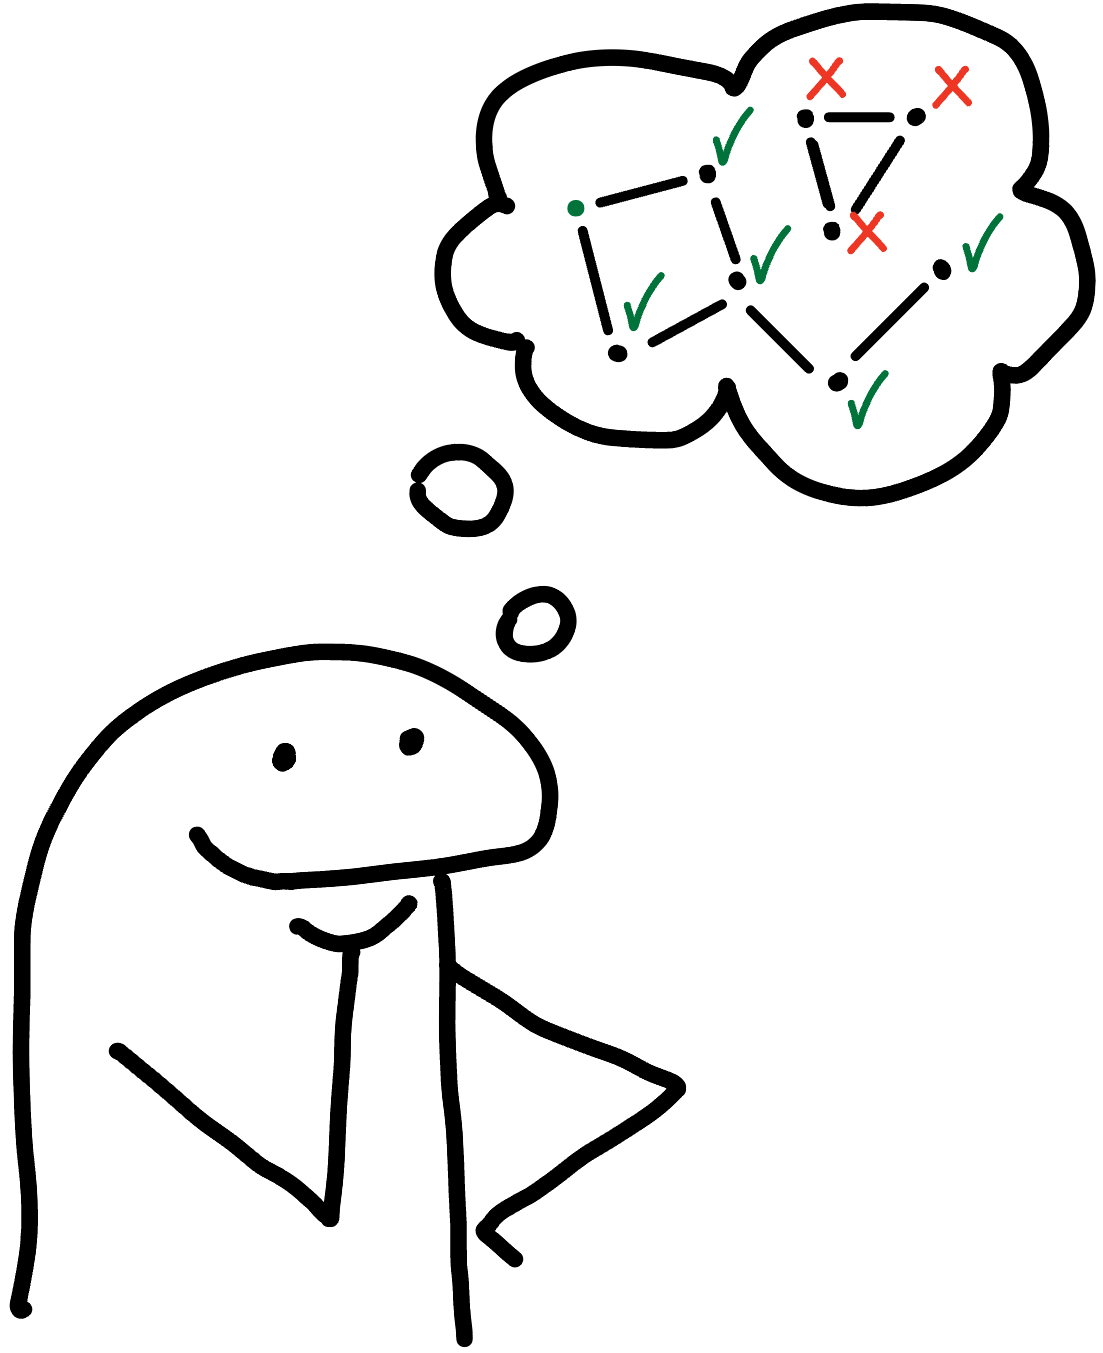
\includegraphics[width=0.8\textwidth]{pic/reachableAns.jpg}
    \end{column}
    \begin{column}{0.35\textwidth}
    \end{column}
    \begin{column}{0.35\textwidth}
    \end{column} 
  \end{columns}

\begin{textblock*}{0.30\textwidth}(0.1\textwidth,0.65\textheight)
\begin{lstlisting}[language=imperative]
procedure DFS(G, v) = 
  S.push(v)
  while !S.empty do
    v = S.pop()
    if (!seen[v]) then
      seen.add(v)
      for (_, w) in G.edges(v) do 
        S.push(w)
\end{lstlisting}
\end{textblock*}
\end{frame}
\addtocounter{framenumber}{-1}

\begin{frame}[fragile]
  \frametitle{No \mk~--- One Task, One Program}
  \begin{columns}    
    \begin{column}{0.35\textwidth}
      \centering
      \vspace{2cm}
      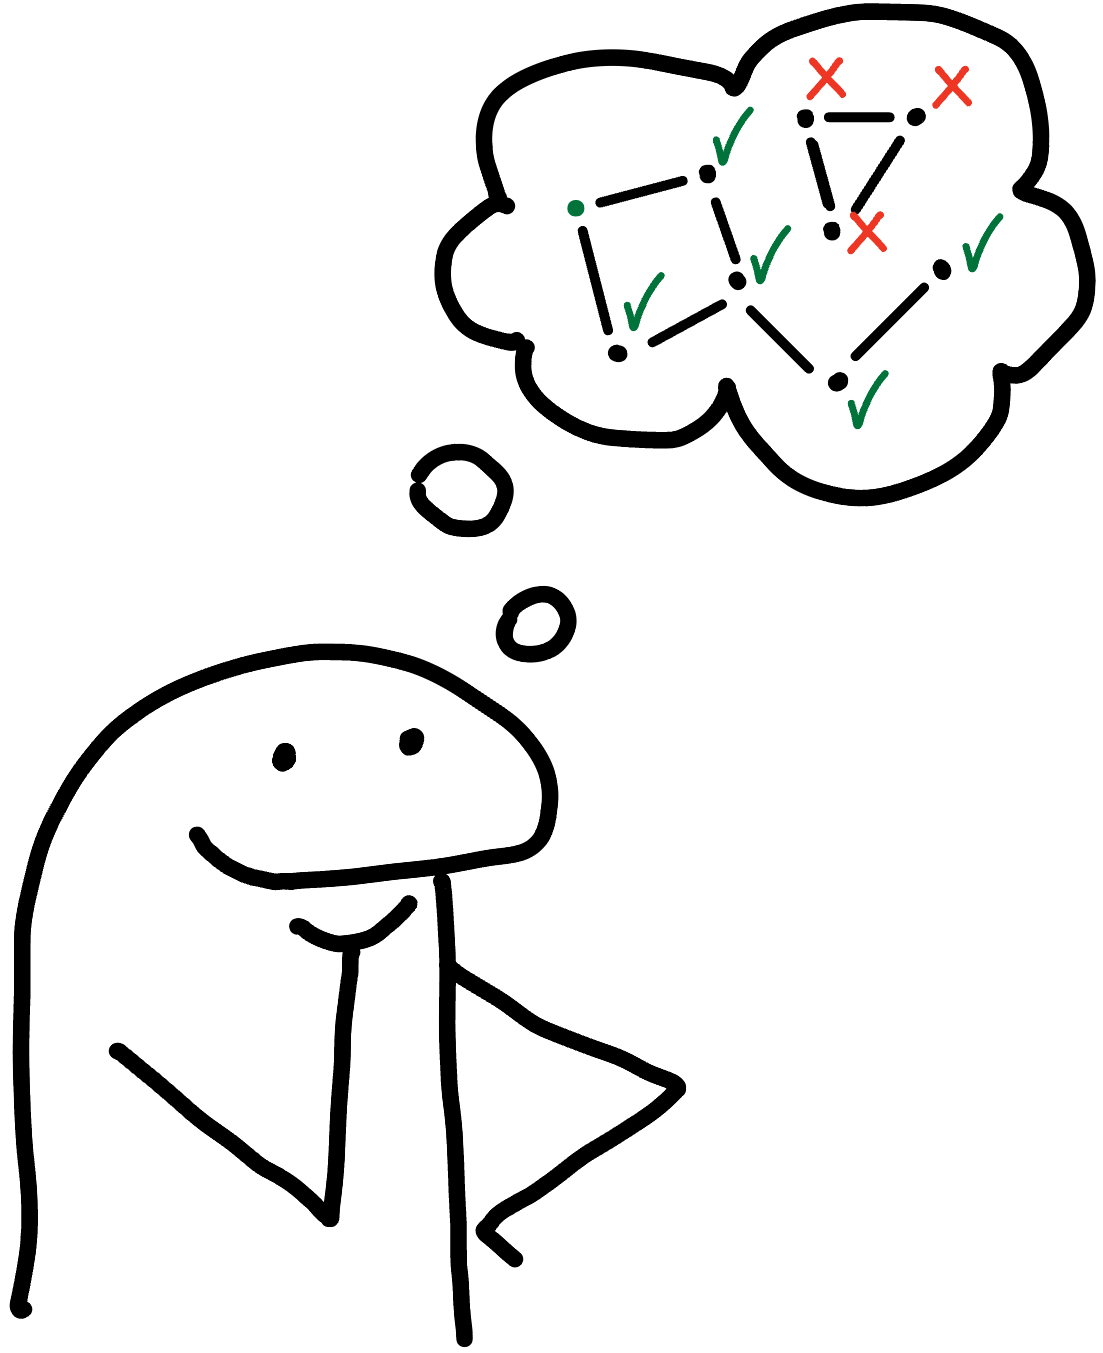
\includegraphics[width=0.8\textwidth]{pic/reachableAns.jpg}
    \end{column}
    \begin{column}{0.35\textwidth}
      \centering
      \vspace{2cm}
      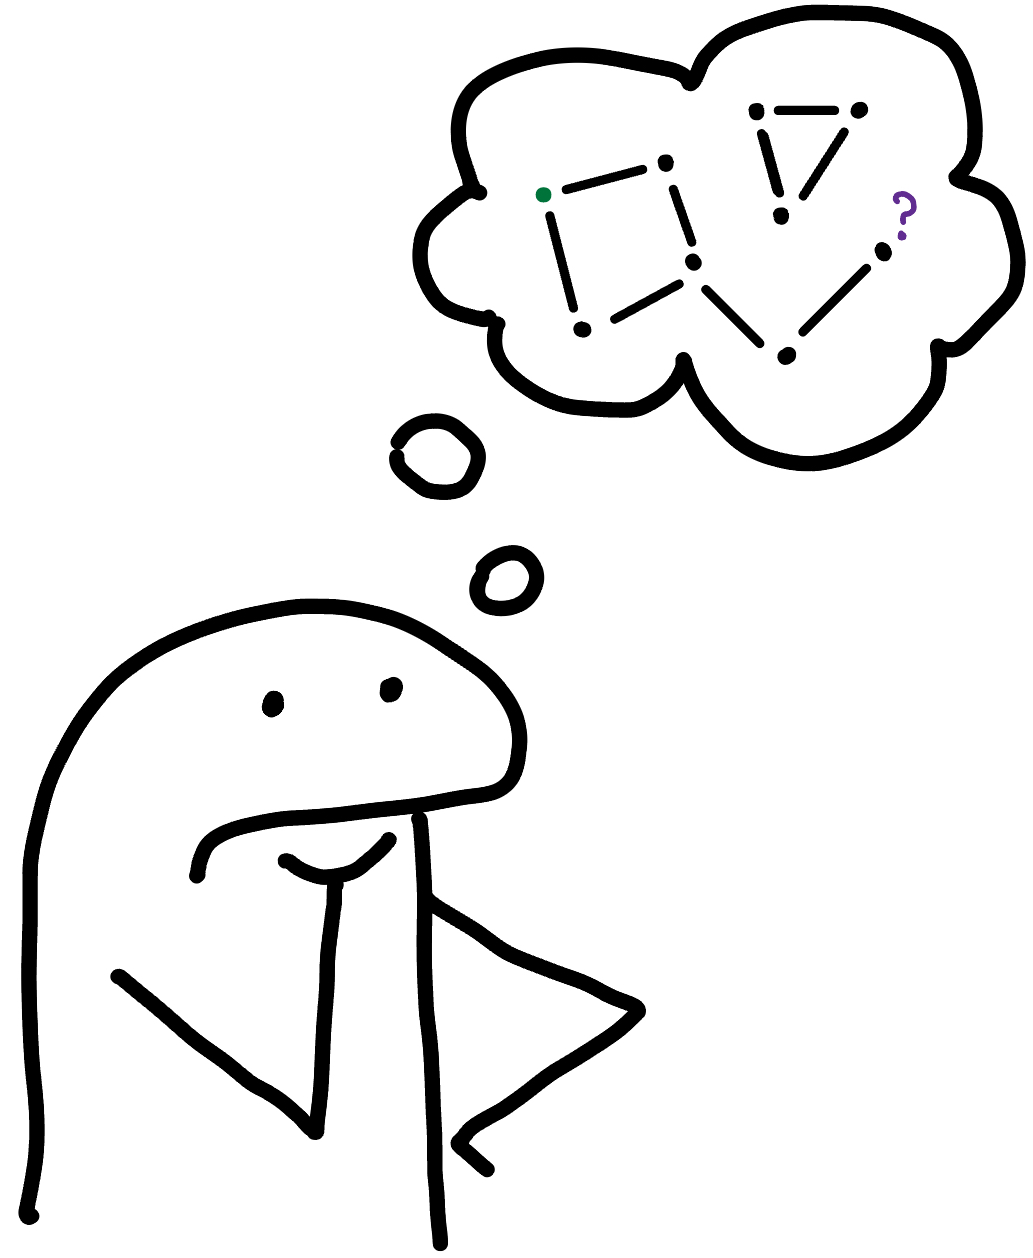
\includegraphics[width=0.8\textwidth]{pic/path.jpg}
    \end{column}
    \begin{column}{0.35\textwidth}
    \end{column} 
  \end{columns}

\begin{textblock*}{0.30\textwidth}(0.1\textwidth,0.65\textheight)
\begin{lstlisting}[language=imperative]
procedure DFS(G, v) = 
  S.push(v)
  while !S.empty do
    v = S.pop()
    if (!seen[v]) then
      seen.add(v)
      for (_, w) in G.edges(v) do 
        S.push(w)
\end{lstlisting}
\end{textblock*}
\end{frame}
\addtocounter{framenumber}{-1}

\begin{frame}[fragile]
  \frametitle{No \mk~--- One Task, One Program}
  \begin{columns}    
    \begin{column}{0.35\textwidth}
      \centering
      \vspace{2cm}
      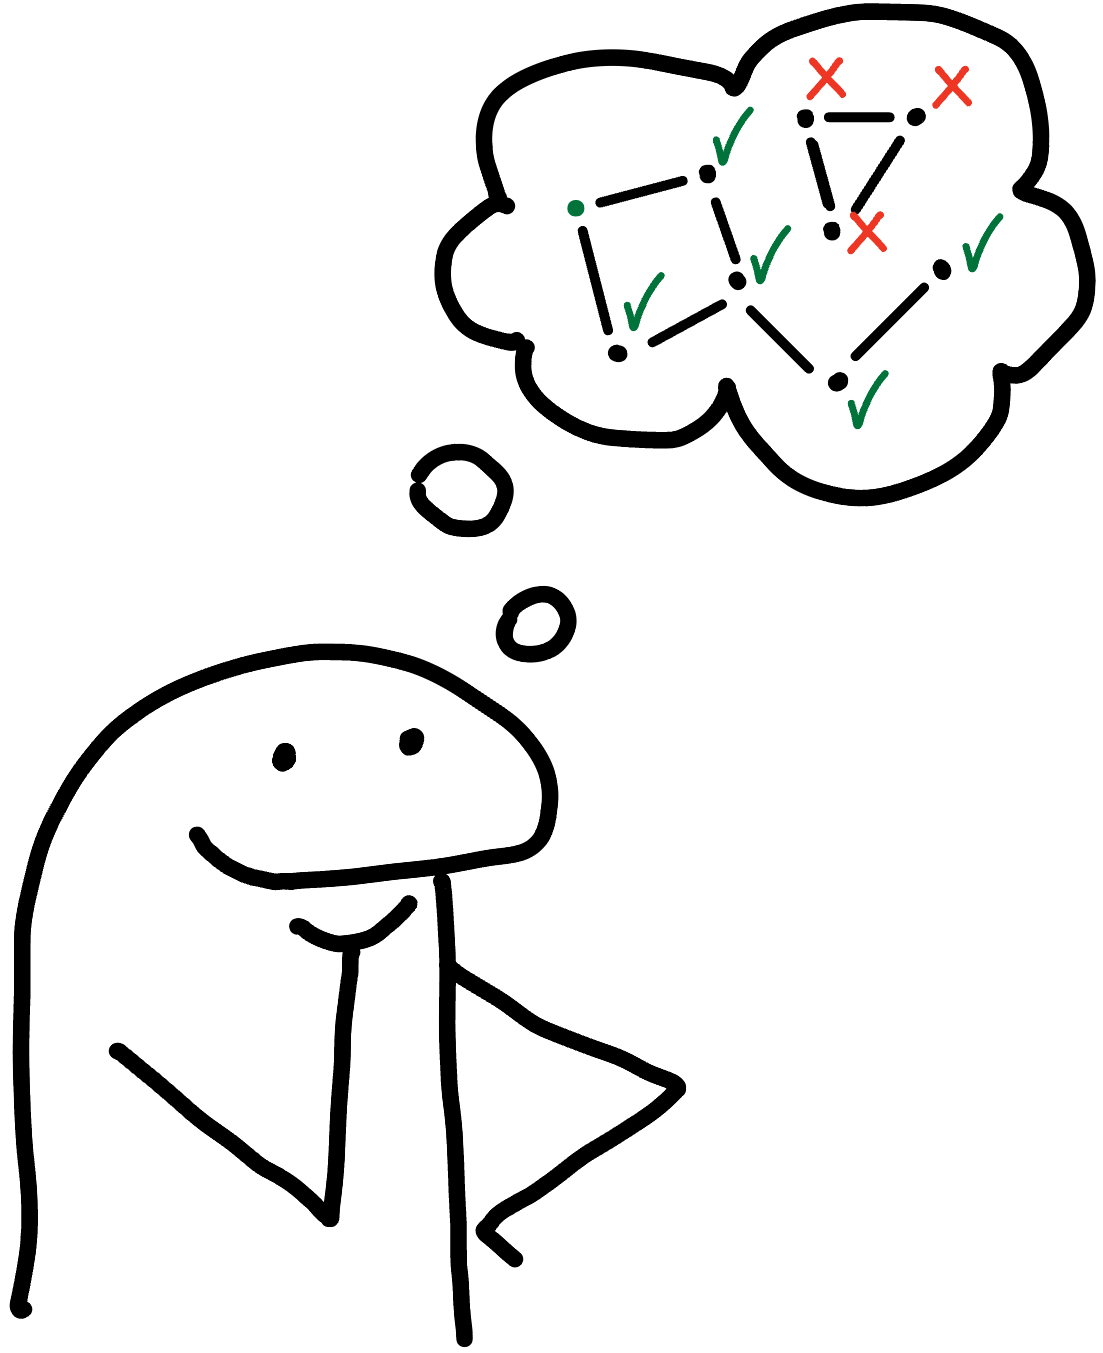
\includegraphics[width=0.8\textwidth]{pic/reachableAns.jpg}
    \end{column}
    \begin{column}{0.35\textwidth}
      \centering
      \vspace{2cm}
      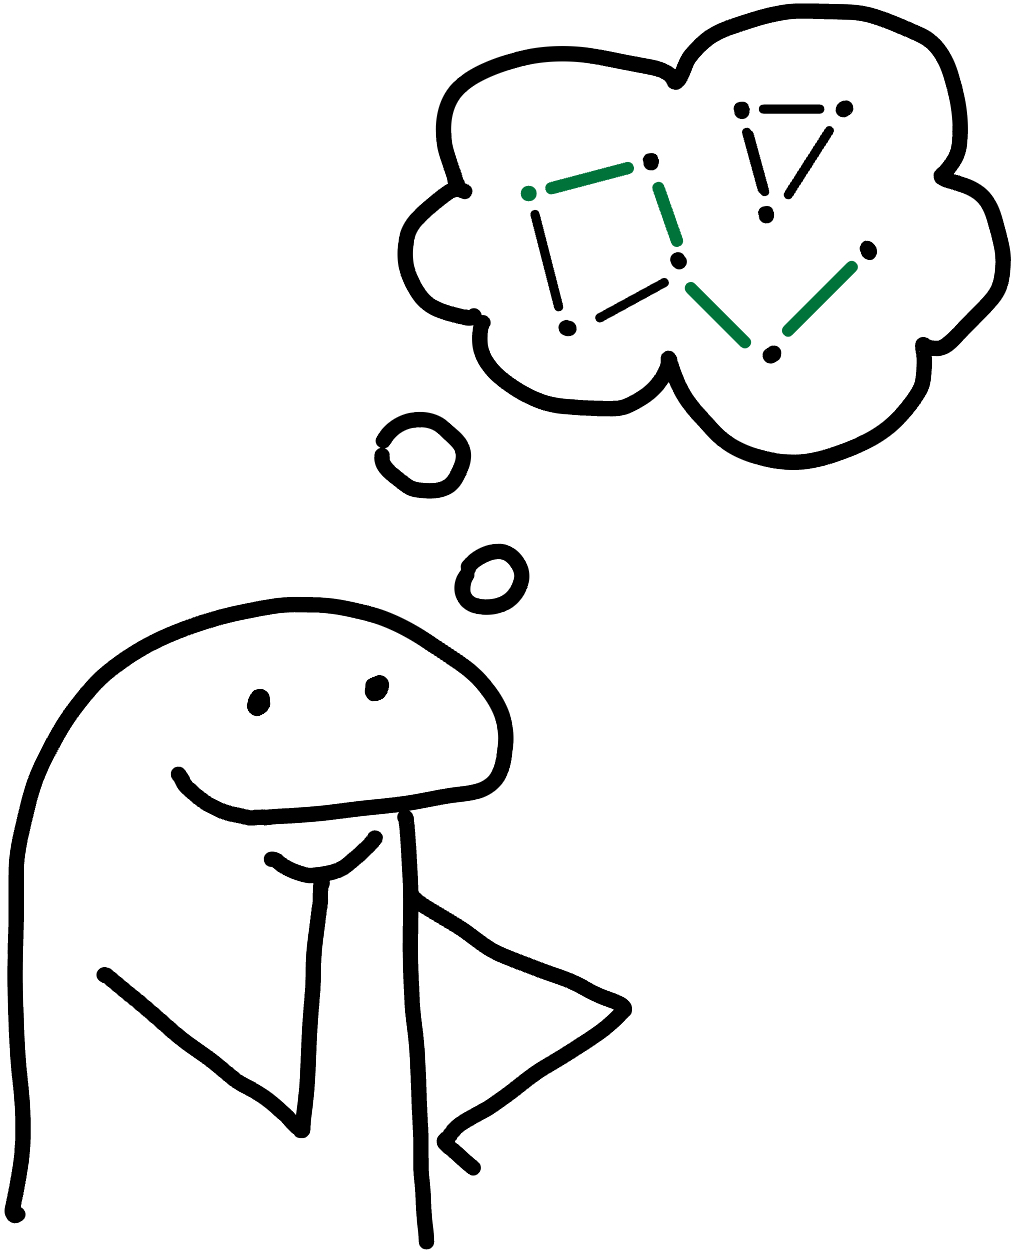
\includegraphics[width=0.8\textwidth]{pic/pathAns.jpg}
    \end{column}
    \begin{column}{0.35\textwidth}
    \end{column} 
  \end{columns}

\begin{textblock*}{0.30\textwidth}(0.1\textwidth,0.65\textheight)
\begin{lstlisting}[language=imperative]
procedure DFS(G, v) = 
  S.push(v)
  while !S.empty do
    v = S.pop()
    if (!seen[v]) then
      seen.add(v)
      for (_, w) in G.edges(v) do 
        S.push(w)
\end{lstlisting}
\end{textblock*}

\begin{textblock*}{0.30\textwidth}(0.45\textwidth,0.65\textheight)
\begin{lstlisting}[language=imperative]
procedure DFS(G, v, u) = 
  path = [v] 
  S.push(v, path)
  while !S.empty do
    (v, path) = S.pop()
    if (v == u) then return path
    if (!seen[v]) then
      seen.add(v)
      for (_, w) in G.edges(v) do 
        S.push((w, path.add(w)))
    return none
\end{lstlisting}
\end{textblock*}
\end{frame}
\addtocounter{framenumber}{-1}


\begin{frame}[fragile]
  \frametitle{No \mk~--- One Task, One Program}
  \begin{columns}    
    \begin{column}{0.35\textwidth}
      \centering
      \vspace{2cm}
      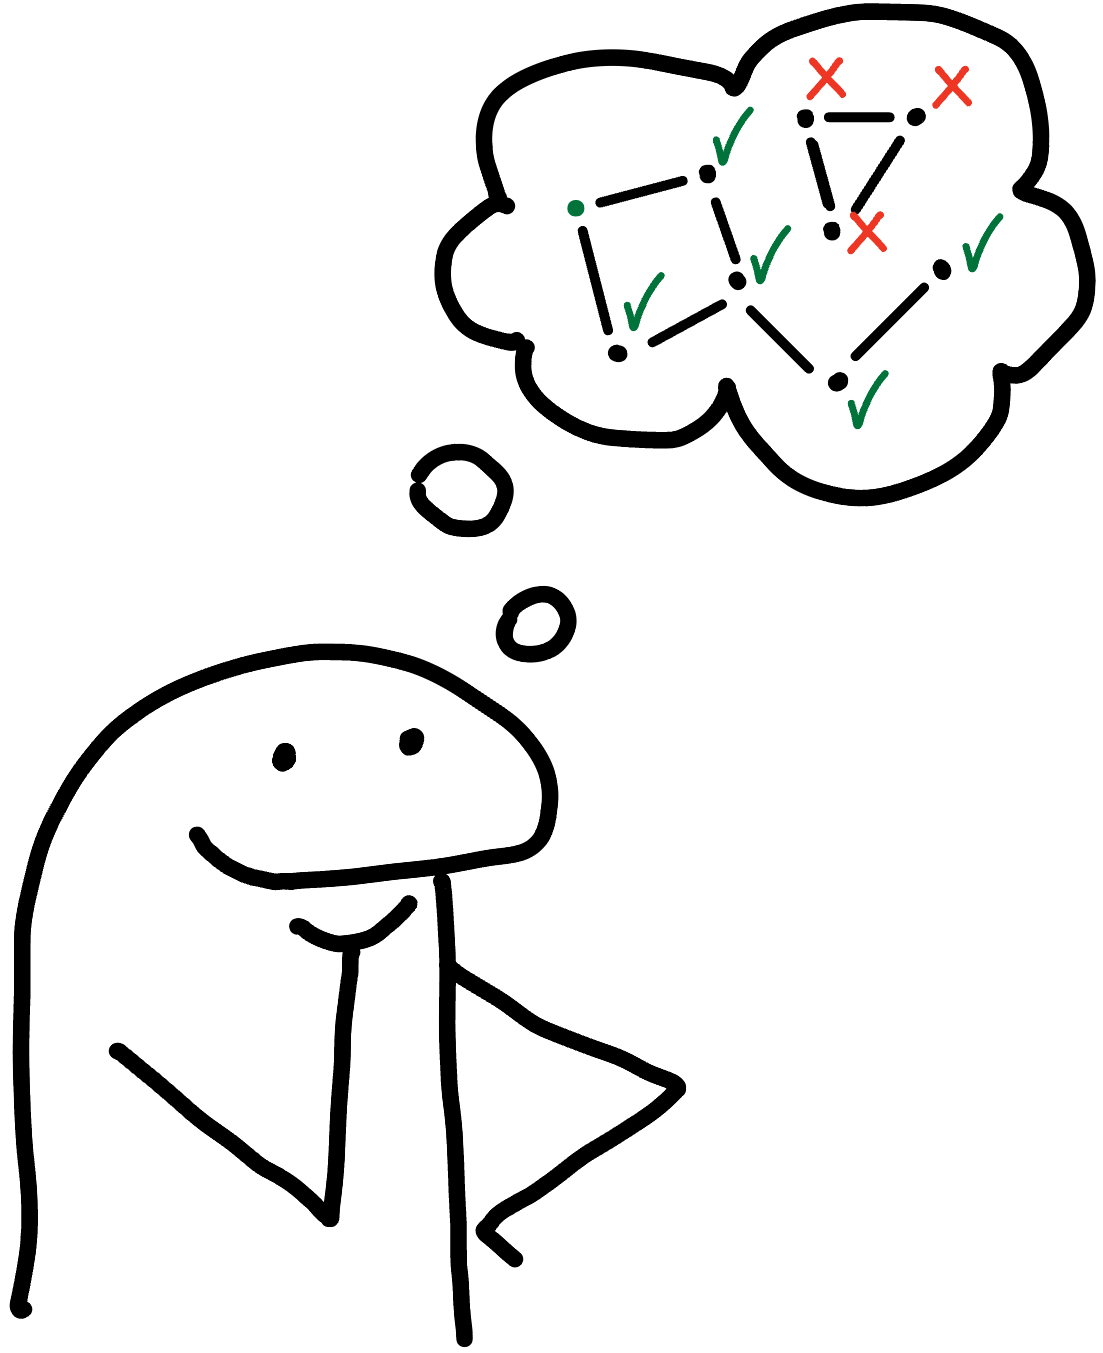
\includegraphics[width=0.8\textwidth]{pic/reachableAns.jpg}
    \end{column}
    \begin{column}{0.35\textwidth}
      \centering
      \vspace{2cm}
      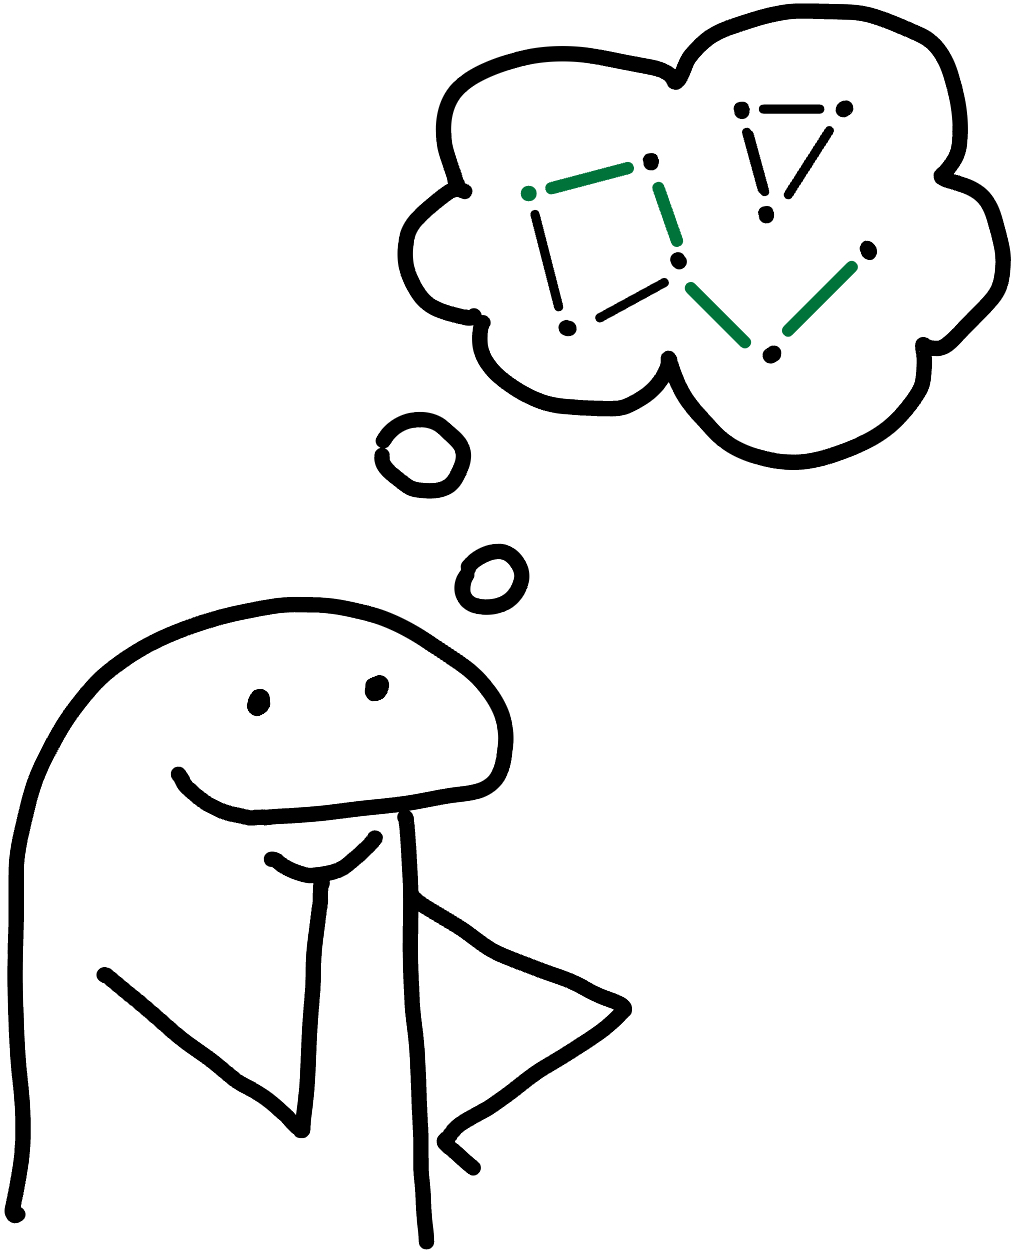
\includegraphics[width=0.8\textwidth]{pic/pathAns.jpg}
    \end{column}
    \begin{column}{0.35\textwidth}
      \centering
      \vspace{2cm}
      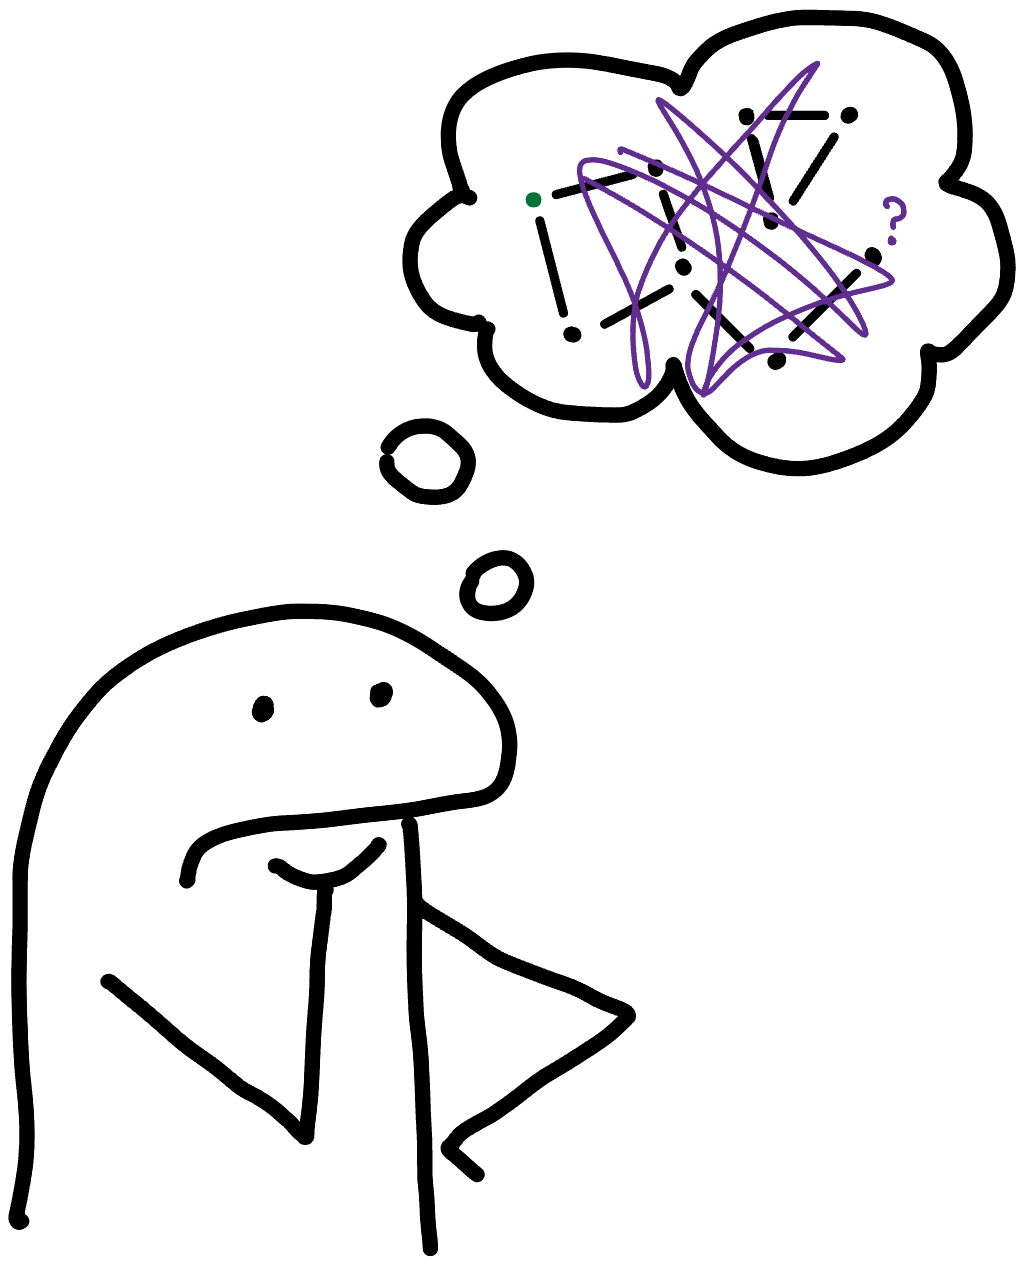
\includegraphics[width=0.8\textwidth]{pic/allPaths.jpg}
    \end{column} 
  \end{columns}

\begin{textblock*}{0.30\textwidth}(0.1\textwidth,0.65\textheight)
\begin{lstlisting}[language=imperative]
procedure DFS(G, v) = 
  S.push(v)
  while !S.empty do
    v = S.pop()
    if (!seen[v]) then
      seen.add(v)
      for (_, w) in G.edges(v) do 
        S.push(w)
\end{lstlisting}
\end{textblock*}

\begin{textblock*}{0.30\textwidth}(0.45\textwidth,0.65\textheight)
\begin{lstlisting}[language=imperative]
procedure DFS(G, v, u) = 
  path = [v] 
  S.push(v, path)
  while !S.empty do
    (v, path) = S.pop()
    if (v == u) then return path
    if (!seen[v]) then
      seen.add(v)
      for (_, w) in G.edges(v) do 
        S.push((w, path.add(w)))
    return none
\end{lstlisting}
\end{textblock*}
\end{frame}
\addtocounter{framenumber}{-1}

\begin{frame}[fragile]
  \frametitle{With \mk~--- Many Tasks, One Relation}
  \begin{columns}    
    \begin{column}{0.35\textwidth}
      \centering
      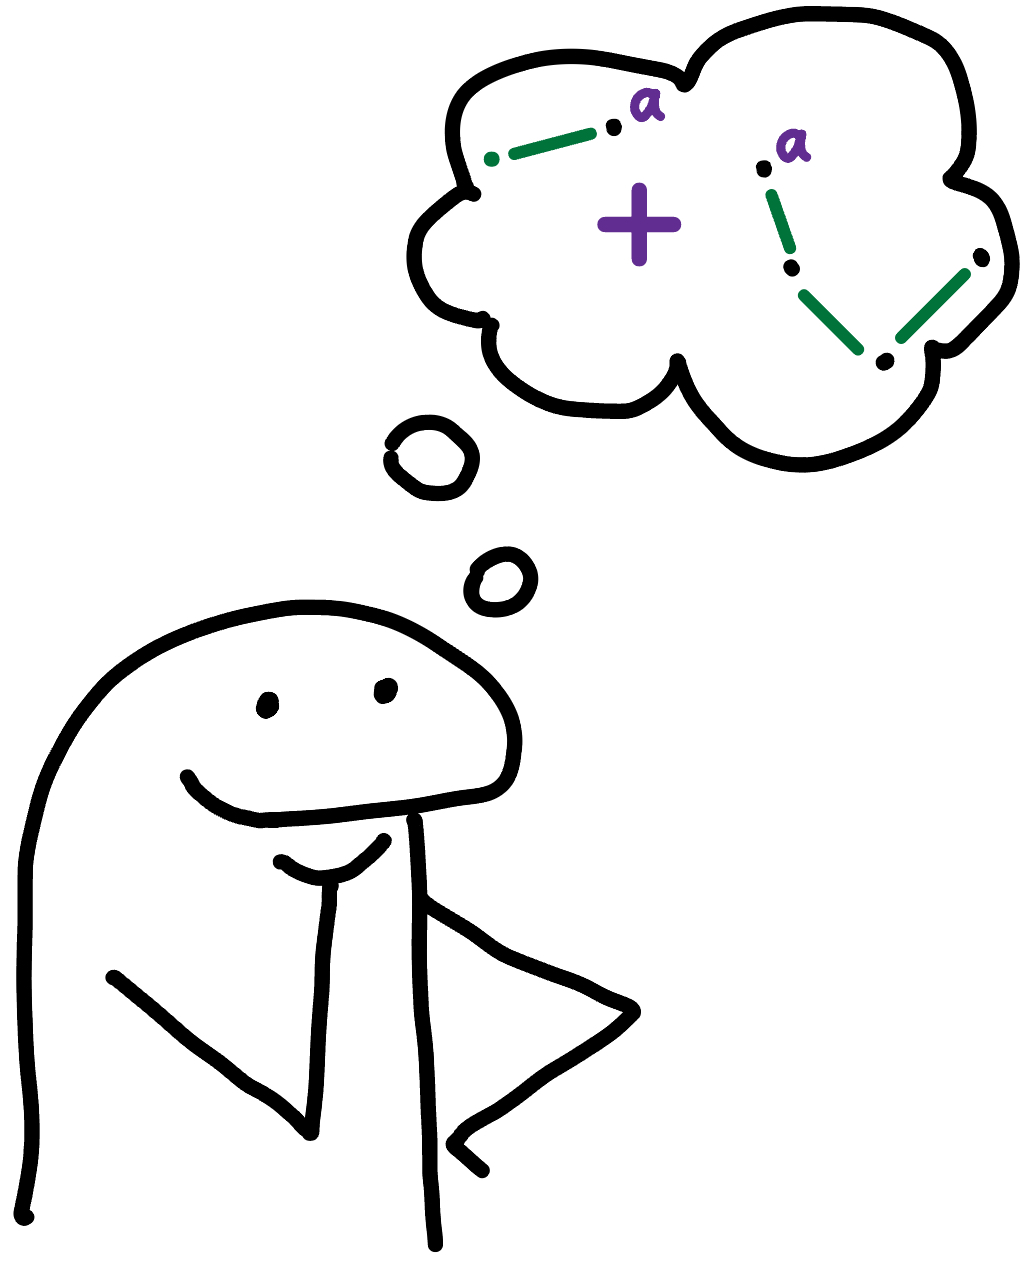
\includegraphics[width=0.8\textwidth]{pic/pathIs.jpg}
    \end{column}
    \begin{column}{0.75\textwidth} 
\[
path(v, u) = 
\begin{cases}
  [v], & \text{if } v = u \\
  v : p,  & \text{if } \exists w: edge(v, w) \wedge p = path(w, u)
\end{cases}
\]

\pause 

\begin{center}
  \begin{minipage}{0.82\textwidth}
\begin{lstlisting}[language=ocanren]
 let rec path$^o$ v u p =                   (* relation *)
   (v === u /\ p === [v]) \/
   (fresh (w p$_1$)
     (edge$^o$ v w /\
      path$^o$ w$_1$ u p$_1$ /\
      p === v : p$_1$) )
\end{lstlisting}
 \pause
    \begin{lstlisting}[language=ocanren]
 run 1 q (path$^o$ A E q)
    \end{lstlisting} \pause
    \begin{lstlisting}[language=ocanren]
 run* q (path$^o$ A E q)
    \end{lstlisting} \pause
    \begin{lstlisting}[language=ocanren]
 run* q (fresh (p) (path$^o$ A q p))
    \end{lstlisting}
 
  \end{minipage}  
\end{center}
    \end{column}
    \end{columns}
\end{frame}


% \begin{frame}[fragile]
%   \frametitle{Relational Programming in \mk}

%   \begin{columns}    
%     \begin{column}{0.35\textwidth}
%       \centering
%       
\includegraphics[width=0.8\textwidth]{pic/edsl.jpg}
%     \end{column}
%     \begin{column}{0.75\textwidth}       
% \begin{center}
%   \begin{minipage}{0.82\textwidth}
%     \begin{lstlisting}[language=racket]
% (define (patho v u p)                 ; Racket
%   (fresh (w p1)
%     (conde
%       [(== v u) (== p `(,v))]
%       [(edge v w)
%        (patho w u p1)
%        (== p (cons v p1))])))

% (run* (q) (patho 'a 'e q))
%     \end{lstlisting}

%     \begin{lstlisting}[language=ocanren]
%  let rec path$^o$ v u p =                      (* OCaml *)
%    (v === u /\ p === [v]) \/
%    (fresh (w p$_1$)
%      (edge$^o$ v w /\
%        path$^o$ w$_1$ u p$_1$ /\
%        p === v : p$_1$) )
%          \end{lstlisting}
%   \end{minipage}
% \end{center}

%       \end{column}
%     \end{columns}
% \end{frame}

\begin{frame}[fragile]
  \frametitle{}

\begin{center}
  \LARGE Solvers from Verifiers
\end{center}

\end{frame}

\begin{frame}[fragile]
  \frametitle{Verifiers}
  \begin{columns}    
    \begin{column}{0.35\textwidth}
      \centering
      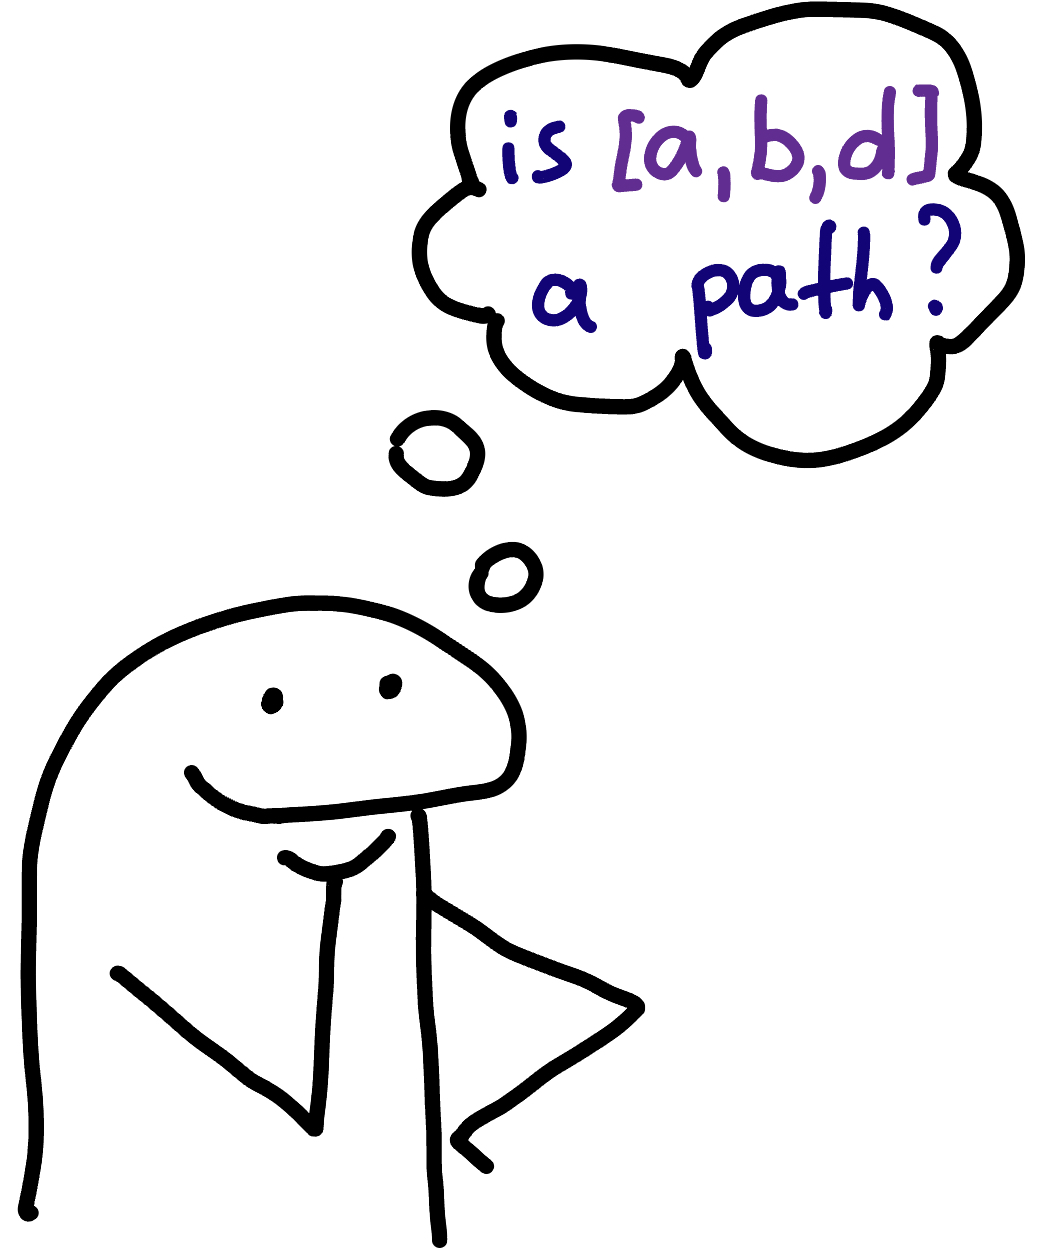
\includegraphics[width=0.8\textwidth]{pic/verifier.jpg}
    \end{column}
    \begin{column}{0.75\textwidth} 
      \begin{center}
        \begin{minipage}{0.82\textwidth}
      \begin{lstlisting}[language=ocanren]
 let rec is_path v u path =             (* function *)
   match path with 
   | [v'] -> v == v' && v == u 
   | v' :: w :: t -> 
       if v == v' && edge v' w 
       then is_path w u (w :: t)
       else false 
      \end{lstlisting}
    \end{minipage}
  \end{center}      
    \end{column}
  \end{columns}
\end{frame}


\begin{frame}[fragile]
  \frametitle{Solvers}
  \begin{columns}    
    \begin{column}{0.35\textwidth}
      \centering
      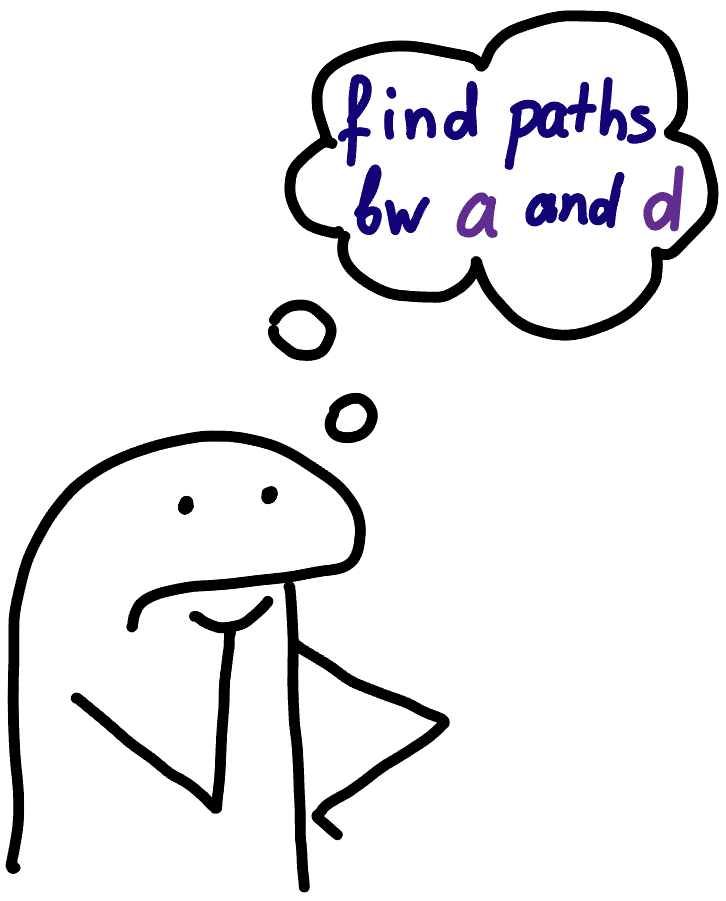
\includegraphics[width=0.8\textwidth]{pic/solver.jpg}
    \end{column}
    \begin{column}{0.75\textwidth} 
      \begin{center}
        \begin{minipage}{0.82\textwidth}
      \begin{lstlisting}[language=ocanren]
  let rec dfs ... = 
    for ... 
      if seen ...
        ... dfs ...  
      ... return ... 
      \end{lstlisting}
    \end{minipage}
  \end{center}      
    \end{column}
  \end{columns}
\end{frame}

\begin{frame}[fragile]
  \frametitle{Solvers from Verifiers}
  \begin{columns}    
    \begin{column}{0.35\textwidth}
      \centering
      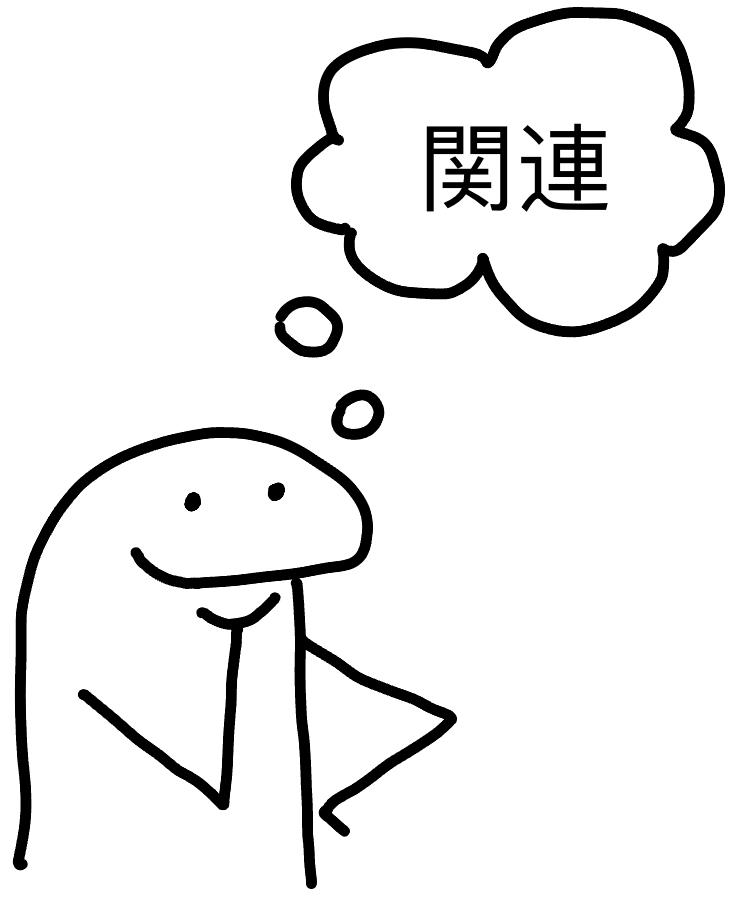
\includegraphics[width=0.8\textwidth]{pic/kanren.jpg}
    \end{column}
    \begin{column}{0.75\textwidth} 
      \vspace{-1cm}
\begin{center}
\begin{tikzpicture}[
  every node/.style = {
    shape=rectangle,
    rounded corners=0.05cm,
    draw,
    align=center,
    minimum size=5mm},
  node distance=1.3em,
  anchor=center
]

\node[inner sep=10pt,draw=none] (function) at (0,0) {
\begin{minipage}{0.82\textwidth}
\begin{lstlisting}[language=ocanren]
 let rec is_path v u path =             (* function *)
   match path with 
   | [v'] -> v == v' && v == u 
   | v' :: w :: t -> 
       if v == v' && edge v' w 
       then is_path w u (w :: t)
       else false 
\end{lstlisting}
\end{minipage}}; 

\node[inner sep=10pt,draw=none] (relation) at (0,-3.5) {
\begin{minipage}{0.82\textwidth}
\begin{lstlisting}[language=ocanren]
 let rec path$^o$ v u p =                   (* relation *)
   (v === u /\ p === [v]) \/
   (fresh (w p$_1$)
     (edge$^o$ v w /\
      path$^o$ w$_1$ u p$_1$ /\
      p === v : p$_1$) )
\end{lstlisting}
\end{minipage}}; 

  \node (unnesting) at ($(relation.north)!0.5!(function.south)$) [draw=none, xshift=-0.1cm] {relational conversion};
  \draw [teal,thick,->] ($(function.south)+(-2,0.5)$) to [out=-90,in=90] ($(relation.north)+(-2,-0.5)$);

  \node (verifier) at ($(relation.center)$) [draw=none, xshift=2cm, yshift=0.5cm,anchor=west] {verifier};
  \draw [teal,thick,->] ($(relation.center)+(-0.5,0)$) to [out=0,in=180] ($(verifier.west)+(0,0)$);

  \node (solver) at ($(relation.center)$) [draw=none, xshift=2cm, yshift=-0.5cm,anchor=west] {solver};
  \draw [teal,thick,->] ($(relation.center)+(-0.5,0)$) to [out=0,in=180] ($(solver.west)+(0,0)$);
  \end{tikzpicture}
\end{center}

    \end{column}
  \end{columns} 
\end{frame}

\begin{frame}[fragile]
  \frametitle{Solvers from Verifiers: Examples}
  \begin{columns}    
    \begin{column}{0.35\textwidth}
      \centering
      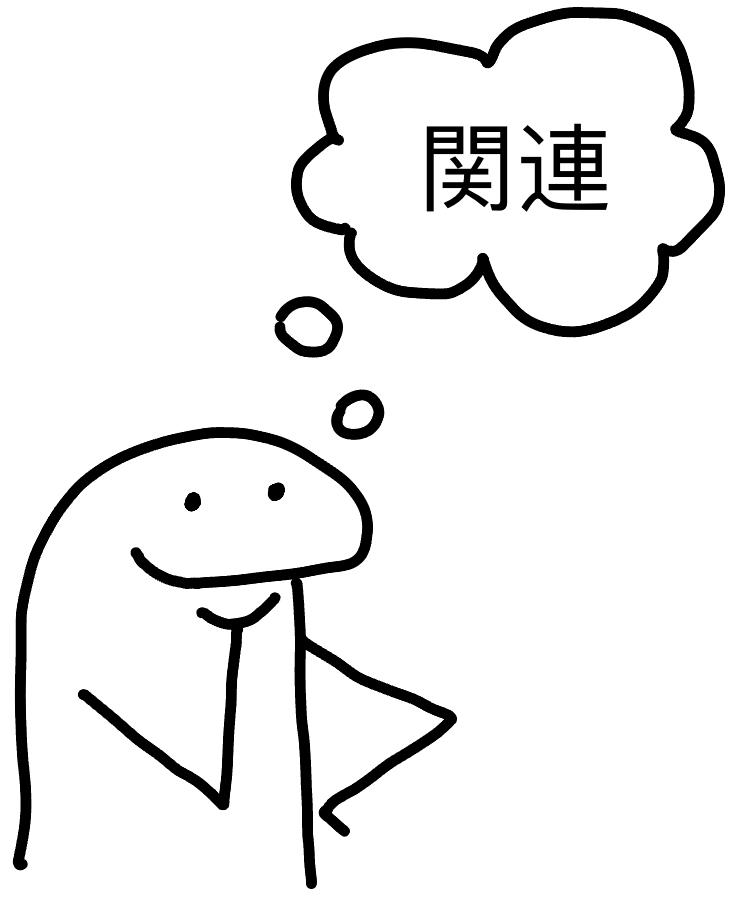
\includegraphics[width=0.8\textwidth]{pic/kanren.jpg}
    \end{column}
    \begin{column}{0.75\textwidth} 
\begin{center}
\begin{tikzpicture}[
  every node/.style = {
    shape=rectangle,
    rounded corners=0.05cm,
    draw,
    align=center,
    minimum size=5mm},
  node distance=1.3em,
  anchor=center
]

\node[draw=none] (evalo) at (0,0) {
\begin{minipage}{0.82\textwidth}
\begin{lstlisting}[language=ocanren]
 let rec eval$^o$ st fm u = 
   fresh (x y v w z) 
     (fm === Conj x y /\
      eval$^o$ st x v /\
      eval$^o$ st y w /\
      and$^o$ v w u) \/
      ... 
\end{lstlisting}
\end{minipage}}; 

\node[draw=none] (typeo) at (0,-3.5) {
\begin{minipage}{0.82\textwidth}
\begin{lstlisting}[language=ocanren]
 let rec type$^o$ e t = 
   (fresh (x y)
     (e === Int x /\ t = TInt) \/
     (e === Plus x y /\
      type$^o$ x Int /\
      type$^o$ y Int /\ 
      t === Int)) \/
      ...  
\end{lstlisting}
\end{minipage}}; 

  \node (evaluation) at ($(evalo.center)$) [draw=none, xshift=1.4cm, yshift=0.5cm,anchor=west] {evaluation};
  \draw [teal,thick,->] ($(evalo.center)+(0,0)$) to [out=0,in=180] ($(evaluation.west)+(0,0)$);

  \node (generation) at ($(evalo.center)$) [draw=none, xshift=1.4cm, yshift=-0.5cm,anchor=west] {program generation};
  \draw [teal,thick,->] ($(evalo.center)+(0,0)$) to [out=0,in=180] ($(generation.west)+(0,0)$);


  \node (typeCheck) at ($(typeo.center)$) [draw=none, xshift=1.4cm, yshift=1cm,anchor=west] {type checking};
  \draw [teal,thick,->] ($(typeo.center)+(0,0)$) to [out=0,in=180] ($(typeCheck.west)+(0,0)$);

  \node (typeInf) at ($(typeo.center)$) [draw=none, xshift=1.4cm, yshift=0cm,anchor=west] {type inference};
  \draw [teal,thick,->] ($(typeo.center)+(0,0)$) to [out=0,in=180] ($(typeInf.west)+(0,0)$);

  \node (typeInh) at ($(typeo.center)$) [draw=none, xshift=1.4cm, yshift=-1cm,anchor=west] {type inhabitance};
  \draw [teal,thick,->] ($(typeo.center)+(0,0)$) to [out=0,in=180] ($(typeInh.west)+(0,0)$);
  \end{tikzpicture}
\end{center}

    \end{column}
  \end{columns}
\end{frame}


\begin{frame}[fragile]
  \frametitle{The Issue}
  \begin{columns}    
    \begin{column}{0.35\textwidth}
      \centering
      
\includegraphics[width=0.8\textwidth]{pic/slow.jpg}
    \end{column} \pause
    \begin{column}{0.75\textwidth} 
    \begin{itemize}
      \item Unifications are expensive
      \item The order of conjunctions is finicky
      \item But! We know something that can help
    \end{itemize}
    \end{column}
  \end{columns}

\end{frame}

\begin{frame}[fragile]
  \frametitle{}

\begin{center}
  \LARGE Specialization
\end{center}

\end{frame}


\begin{frame}[fragile]
  \frametitle{Specialization}

  \begin{columns}    
    \begin{column}{0.35\textwidth}
      \centering
      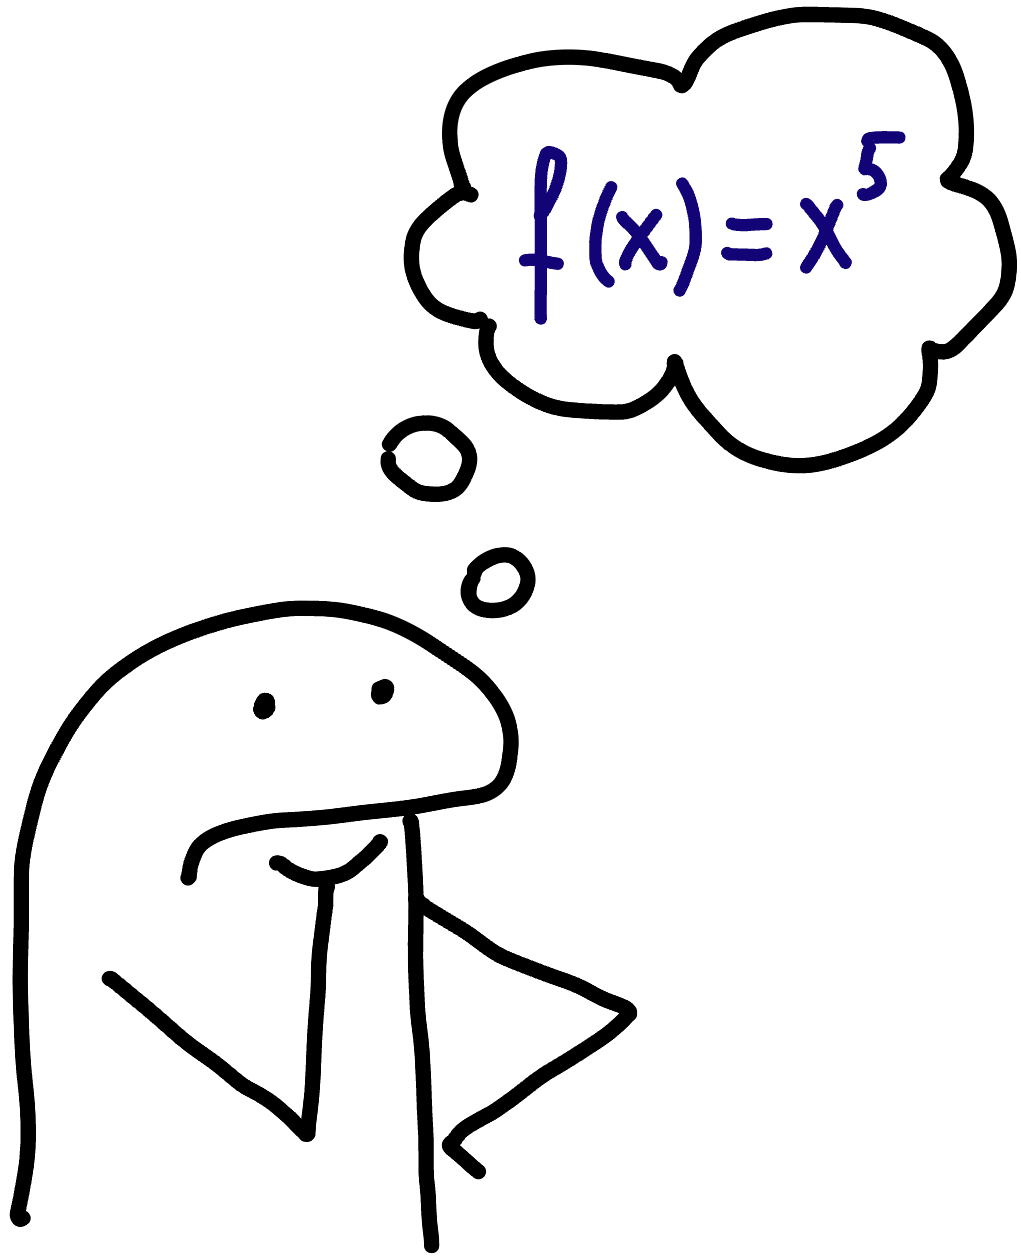
\includegraphics[width=0.8\textwidth]{pic/power.jpg}
    \end{column}
    \begin{column}{0.75\textwidth} 
      \begin{lstlisting}[language=ocanren]
 let rec power base exp = 
   if exp == 0 
   then 1 
   else base * power base (exp - 1)
          \end{lstlisting}

          \begin{lstlisting}[language=ocanren]
 let rec power_5 base =                    (* power base 5 *)
   base * base * base * base * base 
           \end{lstlisting}
        \end{column}
        \end{columns}

\end{frame}

\begin{frame}[fragile]
  \frametitle{Specialization}

  \begin{columns}    
    \begin{column}{0.35\textwidth}
      \centering
      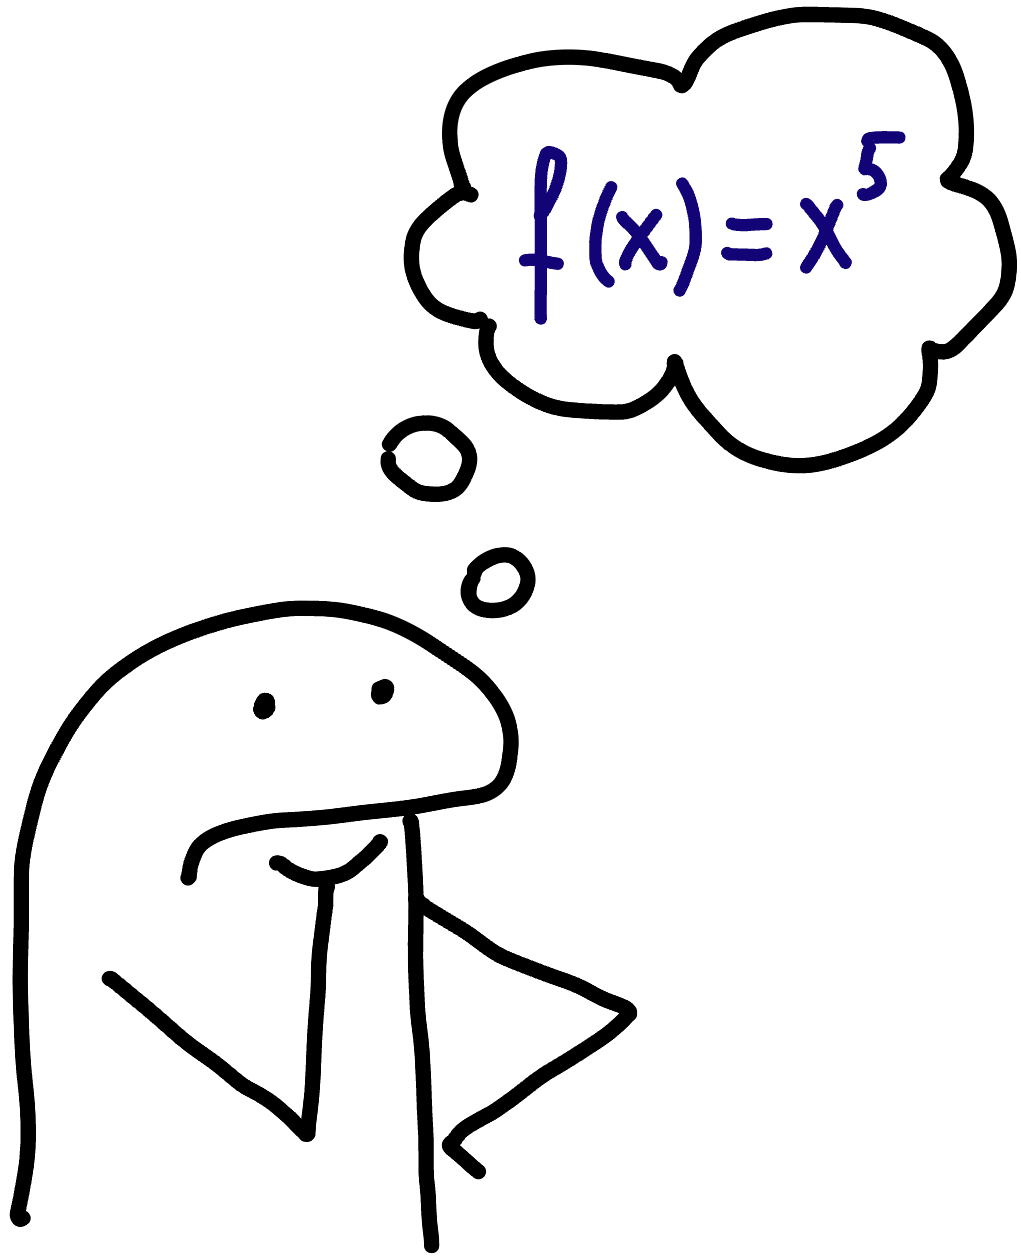
\includegraphics[width=0.8\textwidth]{pic/power.jpg}
    \end{column}
    \begin{column}{0.75\textwidth} 
\[
  program: I_{static} \times I_{dynamic} \to O 
\]

\[
  program_{I_{static}}: I_{dynamic} \to O 
\]

\vspace{0.5cm}

\begin{center}
  Same outputs for the same inputs
\end{center}
        \end{column}
        \end{columns}

\end{frame}


\begin{frame}[fragile]
  \frametitle{Static Data in \mk: Modes}
  \begin{columns}    
    \begin{column}{0.35\textwidth}
      \centering
      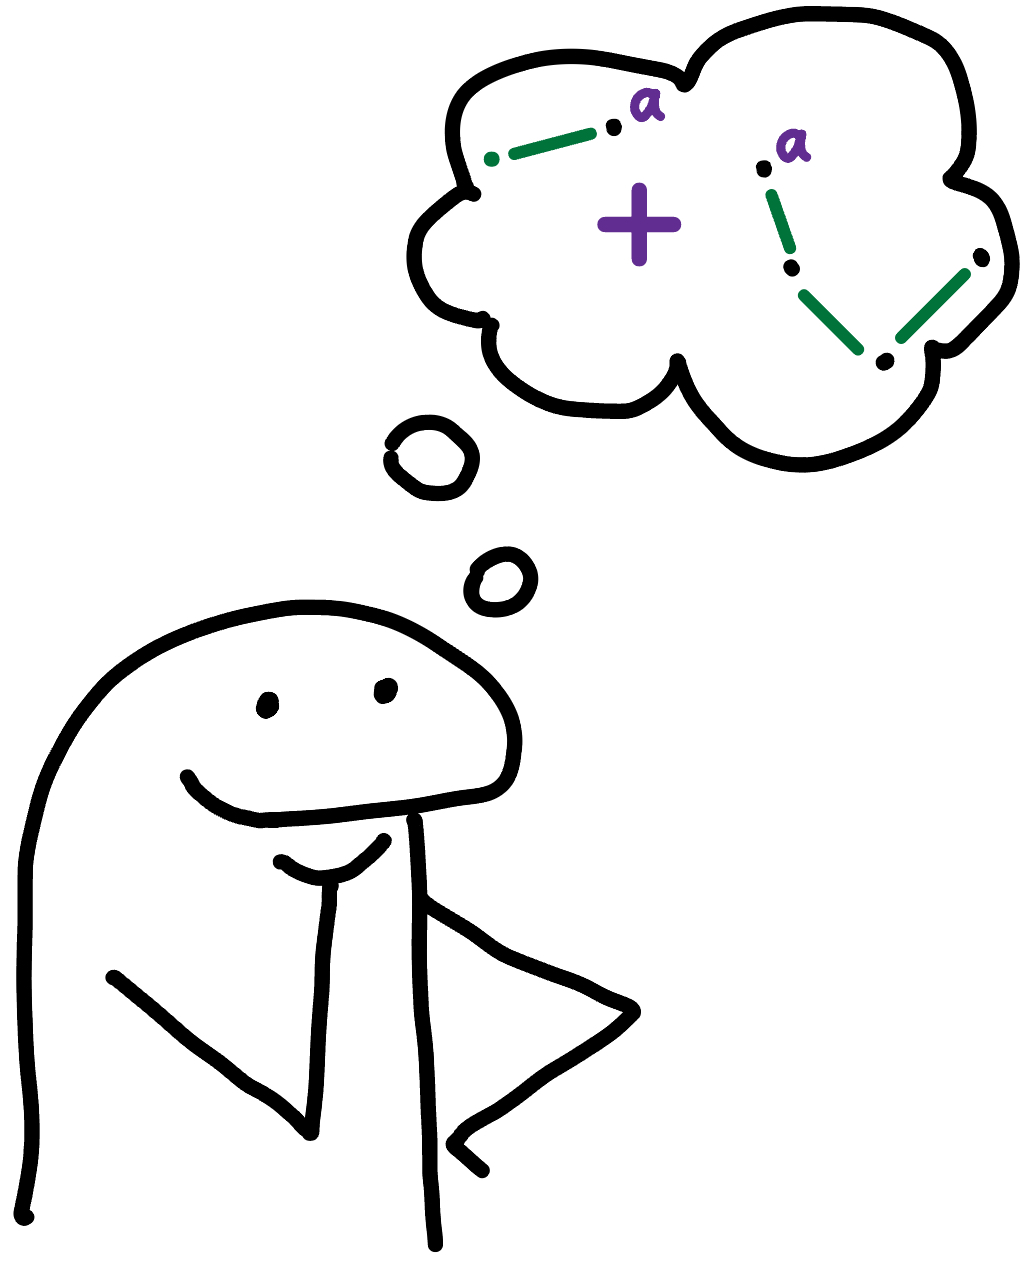
\includegraphics[width=0.8\textwidth]{pic/pathIs.jpg}
    \end{column}
    \begin{column}{0.75\textwidth} 
\begin{center}
  \begin{minipage}{0.82\textwidth}
First two arguments known (mode \texttt{in in out})
    \begin{lstlisting}[language=ocanren]
 run* q (path$^o$ A E p)
    \end{lstlisting} 
\pause 
\vspace{1cm}

Last argument known (mode \texttt{out out in})

    \begin{lstlisting}[language=ocanren]
 run* (p q) (path$^o$ p q [A, B, C, D, E])
    \end{lstlisting} 

\pause 
\vspace{1cm}

Arguments may not be known (mode \texttt{in out out})

    \begin{lstlisting}[language=ocanren]
run* (q) (fresh (p) (path$^o$ A q p))
    \end{lstlisting}

  \end{minipage}  
\end{center}
    \end{column}
    \end{columns}

\end{frame}

% \begin{frame}[fragile]
%   \frametitle{Evaluator of Logic Formulas: Order of Calls}
%   \begin{tikzpicture}[remember picture, overlay]

%     \node (a) [
%       program,
%       anchor=north,
%       yshift=-1.8cm
%     ]
%     at (current page.north)
%     {
%       \adjustbox{scale=0.8}
%       {
%         \begin{minipage}[c]{\textwidth}
%           \lstset{language=ocanren1}

\begin{lstlisting}
let rec eval$^o$ fm s r =
  fresh (v x y a b) (
    (fm === var v /\ lookup$^o$ v s r) \/
    (fm === neg x /\ eval$^o$ x s a /\ not$^o$ a r) \/
    (fm === conj x y /\ eval$^o$ x s a /\ eval$^o$ y s b /\ and$^o$ a b r) \/
    (fm === disj x y /\ eval$^o$ x s a /\ eval$^o$ y s b /\ or$^o$ a b r) )
  \end{lstlisting}
%         \end{minipage}
%       }
%     };

%     \node (b) [
%       transparent,
%       anchor=south]
%       at (a.north)
%     {\footnotesize
%         boolean connective last
%     };

%     \node[draw=none, fill=green!50, opacity=0.2, shape=rectangle, minimum width=1.3cm,minimum height=0.45cm, anchor=west] at ($(a.south)+(-0.85,1.3)$) {};
%     \node[draw=none, fill=green!50, opacity=0.2, shape=rectangle, minimum width=1.7cm,minimum height=0.9cm, anchor=west] at ($(a.south)+(1.75,0.7)$) {};


%     \node (c) [
%       program,
%       anchor=south,
%       yshift=0.8cm
%     ]
%     at (current page.south)
%     {
%       \adjustbox{scale=0.8}
%       {
%         \begin{minipage}[c]{\textwidth}
%           \lstset{language=ocanren1}

\begin{lstlisting}
let rec eval$^o$ fm s r =
  fresh (v x y a b)
    (fm === var v /\ lookup$^o$ v s r) \/
    (fm === neg x /\ not$^o$ a r /\ eval$^o$ x s a) \/
    (fm === conj x y /\ and$^o$ a b r /\ eval$^o$ x s a /\ eval$^o$ y s b) \/
    (fm === disj x y /\ or$^o$ a b r /\ eval$^o$ x s a /\ eval$^o$ y s b) }
  \end{lstlisting}
%         \end{minipage}
%       }
%     };

%     \node[draw=none, fill=green!50, opacity=0.2, shape=rectangle, minimum width=1.3cm,minimum height=0.45cm, anchor=west] at ($(c.south)+(-3.05,1.35)$) {};
%     \node[draw=none, fill=green!50, opacity=0.2, shape=rectangle, minimum width=1.7cm,minimum height=0.85cm, anchor=west] at ($(c.south)+(-2.6,0.7)$) {};


%     \node (d) [
%       transparent,
%       anchor=south]
%       at (c.north)
%     {\footnotesize
%       boolean connective first
%     };
%     \onslide<1->
%   \end{tikzpicture}

% \end{frame}

% \begin{frame}[fragile]
%   \frametitle{Evaluator of Logic Formulas: Evaluation}
% \begin{table}[!h]
%   \resizebox{0.65\textwidth}{!}{
%     \begin{minipage}{\textwidth}
%       \centering
%       \begin{tabular}{c||c||c}
%                         & Implementation & Placement \\ \hline\hline
%       \emph{FirstPlain} & table-based    & before \\ \hline
%       \emph{LastPlain}  & table-based    & after  \\ \hline
%       \emph{FirstNando} & via nand$^o$   & before \\ \hline
%       \emph{LastNando}  & via nand$^o$   & after  \\
%       \end{tabular}
%       \caption{Different implementations of eval$^o$}
%     \end{minipage}
%   }
% \label{tbl:eval}
% \end{table}

% \begin{center}
%   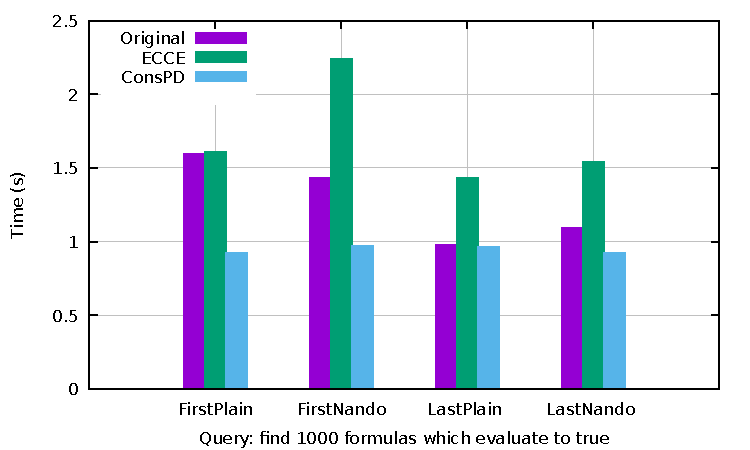
\includegraphics[width=0.45\textwidth]{fig/prop/prop.pdf}
% \end{center}
% \end{frame}

\begin{frame}[fragile]
  \frametitle{Optimal Conjunction Order Depends on a Mode}
\begin{columns}
  \begin{column}[t]{0.49\textwidth}
    
\lstset{moredelim=[is][\bfseries]{[*}{*]}}

\begin{figure}[h]
  \centering
  \begin{minipage}{0.65\columnwidth}
    \begin{lstlisting}[frame=tb,language=ocanren1]
 let rec sort$^o$ x y =
   (x === [] /\ y === []) \/ 
   (fresh (s xs xs$_1$)
     y === s :: xs$_1$ /\
     smallest$^o$ x s xs /\
     sort$^o$ xs xs$_1$)
    \end{lstlisting}
  \end{minipage}
\end{figure}


    \vfill

    \begin{center}
      \begin{minipage}{0.4\textwidth}
        \begin{itemize}
          \item[\happyCheck] sorting
          \item[\timeout] permutations
        \end{itemize}
      \end{minipage}
    \end{center}

  \end{column}
  \begin{column}[t]{0.49\textwidth}
    
\lstset{moredelim=[is][\bfseries]{[*}{*]}}

\begin{figure}[h]
  \centering
  \begin{minipage}{0.65\columnwidth}
    \begin{lstlisting}[frame=tb,language=ocanren1]
 let rec sort$^o$ x y = 
   (x === [] /\ y === []) \/
   (fresh (s xs xs$_1$)
     y === s :: xs$_1$ /\
     sort$^o$ xs xs$_1$ /\
     smallest$^o$ x s xs)
    \end{lstlisting}
  \end{minipage}
\end{figure}
 

    \vfill

    \begin{center}
      \begin{minipage}{0.4\textwidth}
        \begin{itemize}
          \item[\timeout] sorting
          \item[\happyCheck] permutations
        \end{itemize}
      \end{minipage}
    \end{center}


  \end{column}
\end{columns}
\end{frame}

\begin{frame}[fragile]
  \frametitle{}
\begin{center}
  \LARGE Functional Conversion
\end{center}
\end{frame}

\begin{frame}[fragile]
  \frametitle{Generating Solvers from Verifiers}

\tikzset{
    block/.style={
      rectangle, draw, minimum width = 2.5cm, minimum height=1.5cm, align=center
        },
}

\newcommand{\fTo}[2]{
  \draw[-Stealth,thick,color=teal] (#1) -- (#2);
}

\begin{center}
  \begin{tikzpicture}[
    every node/.style = {
        inner sep=0pt
      , shape=rectangle
      }
  ]

      \coordinate (shift) at (2.8,-1.5);  

      \node[block] (relInt) at ($(shift)$) {relational \\ conversion};
      \node[block] (spec) at ($(relInt)+(shift)$) {specialization};
      \node[block] (funCon) at ($(spec)+(shift)$) {functional \\ conversion};

      \node[] (args) at ($(spec.west)!(relInt.south)!(spec.east)$) {args};
      \node[] (dir) at ($(funCon.west)!(spec.south)!(funCon.east)$) {direction};

      \node[] (p_m) at ($(relInt.west)!(spec.north)!(relInt.east)$) {p$^o$};
      \node[] (p_i) at ($(spec.west)!(funCon.north)!(spec.east)$) {p$^s$};

      \node[] (p) at ($(relInt.west)+(-0.6,0)$) {$p$};
    
      \node[anchor=west] (haskell) at ($(funCon.north east)+(1,0)$) {Haskell};
      \node[anchor=west] (ocaml) at ($(funCon.east)+(1,0)$) {OCaml};
      \node[anchor=west] (dots) at ($(funCon.south east)+(1,0)$) { $\ \dots$};

      \fTo{$(relInt.east)$}{p_m};
      \fTo{p_m}{spec.north};

      \fTo{$(spec.east)$}{p_i};
      \fTo{p_i}{funCon.north};

      \fTo{p}{$(relInt.west)$};

      \fTo{args}{$(spec.west)$};

      \fTo{dir}{$(funCon.west)$};


      \fTo{funCon.east}{$(haskell.west)$};
      \fTo{funCon.east}{$(ocaml.west)$};
      \fTo{funCon.east}{$(dots.west)$};

  \end{tikzpicture}
  \end{center}
  
  


\end{frame}


% \begin{frame}[fragile]
%   \frametitle{Example: Addition in the Forward Direction}
% \begin{columns}
%   \begin{column}[t]{0.49\textwidth}
%     \begin{figure}[!t]
  \centering
  \begin{minipage}{0.6\columnwidth}
    \begin{lstlisting}[language=ocanren1,frame=tb]
 let rec add$^o$ x y z = 
   (x === O /\ y === z) \/
   (fresh (x$_1$ z$_1$)
     (x === S x$_1$ /\
      add$^o$ x$_1$ y z$_1$ /\
      z === S z$_1$) )
    \end{lstlisting}
  \end{minipage}
\end{figure}
%     \[ \text{add}^{\circ}\ 0\ 1\ z = \{z \mapsto 1\}\]
%   \end{column}
%   \begin{column}[t]{0.49\textwidth}
%     \begin{figure}[!t]
  \centering
  \begin{minipage}{0.8\columnwidth}
    \begin{lstlisting}[language=ocanren1,frame=tb]
 addIIO $::$ Nat -> Nat -> Nat
 addIIO x y =
   case x of
     O -> y
     S x$_1$ -> S (addIIO x$_1$ y)
    \end{lstlisting}
  \end{minipage}
\end{figure}

%     \[ \text{addIIO}\ 0\ 1 = 1 \] 
%   \end{column}
% \end{columns}
% \end{frame}


\begin{frame}[fragile]
  \frametitle{Addition in the Backward Direction: Nondeterminism}
\begin{columns}
  \begin{column}[t]{0.49\textwidth}
    \begin{figure}[!t]
  \centering
  \begin{minipage}{0.6\columnwidth}
    \begin{lstlisting}[language=ocanren1,frame=tb]
 let rec add$^o$ x y z = 
   (x === O /\ y === z) \/
   (fresh (x$_1$ z$_1$)
     (x === S x$_1$ /\
      add$^o$ x$_1$ y z$_1$ /\
      z === S z$_1$) )
    \end{lstlisting}
  \end{minipage}
\end{figure}
  \end{column}
  \begin{column}[t]{0.49\textwidth}
    \begin{figure}[!t]
  \centering
  \begin{minipage}{0.9\columnwidth}
    \begin{lstlisting}[frame=tb,language=ocanren1]
addOOI $::$ Nat -> Stream (Nat, Nat)
addOOI z =
  return (O, z) <$\mid$>
  case z of
    O -> Empty
    S z$_1$ -> do
      (x$_1$, y) <- addOOI z$_1$
      return (S x$_1$, y)
    \end{lstlisting}
  \end{minipage}
\end{figure}

  \end{column}
\end{columns}

\vfill
$\text{add}^{\circ}\ x\ y\ 1 = \left[\{x \mapsto  0, y \mapsto  1\}, \{x \mapsto  1, y \mapsto  0\} \right]$

\vfill

\lstinline{addOOI 1 = [(0,1), (1,0)]}

\end{frame}

\begin{frame}[fragile]
  \frametitle{Free Variables in Answers: Generators}
\begin{columns}
  \begin{column}[t]{0.49\textwidth}
    \begin{figure}[!t]
  \centering
  \begin{minipage}{0.6\columnwidth}
    \begin{lstlisting}[language=ocanren1,frame=tb]
 let rec add$^o$ x y z = 
   (x === O /\ y === z) \/
   (fresh (x$_1$ z$_1$)
     (x === S x$_1$ /\
      add$^o$ x$_1$ y z$_1$ /\
      z === S z$_1$) )
    \end{lstlisting}
  \end{minipage}
\end{figure}

    \vspace{0.5cm}
    $\text{add}^{\circ}\ 1\ y\ z = \{z \mapsto S\ y\}$

    \vspace{0.5cm}

    \lstinline{genNat = [0, 1, 2, ...]}

    \vspace{0.5cm}

    \lstinline{addIOO 1 = [(0,1), (1,2), (2,3), ...]} 
  \end{column}
  \begin{column}[t]{0.49\textwidth}
    \begin{figure}[h]
\centering
\begin{minipage}{0.9\columnwidth}
  \begin{lstlisting}[frame=tb, language=ocanren1]
addIOO $::$ Nat -> Stream (Nat, Nat)
addIOO x =
  case x of
    O -> do
      z <- genNat
      return (z, z)
    S x$_1$ -> do
      (y, z$_1$) <- addIOO x$_1$
      return (y, S z$_1$)

 genNat $::$ Stream Nat
 genNat = 
    (return O) <$\mid$> (S <$\$$> genNat)
  \end{lstlisting}
\end{minipage}
\end{figure}

  \end{column}
\end{columns}
\end{frame}

\begin{frame}[fragile]
  \frametitle{Old Functional Conversion}
\tikzset{
    block/.style={
      rectangle, draw, minimum width = 2.5cm, minimum height=1.5cm, align=center
        },
}

\newcommand{\fTo}[2]{
  \draw[-Stealth,thick,color=teal] (#1) -- (#2);
}

\begin{center}
  \begin{tikzpicture}[
    every node/.style = {
        inner sep=0pt
      , shape=rectangle
      }
  ]

      \coordinate (shift) at (2.8,-1.5);  


      \node[block] (parser) at ($(shift)$) {parser};
      \node[block] (norm) at ($(parser)+(shift)$) {normalization};
      \node[block] (mode) at ($(norm)+(shift)$) {mode \\ analysis};
      \node[block] (print) at ($(mode)+(shift)$) {pretty \\ printing};

      \node[] (args) at ($(mode.west)!(norm.south)!(mode.east)$) {direction};

      \node[] (ast) at ($(parser.west)!(norm.north)!(parser.east)$) {AST};
      \node[] (p_n) at ($(norm.west)!(mode.north)!(norm.east)$) {p$^n$};
      \node[] (p_m) at ($(mode.west)!(print.north)!(mode.east)$) {p$^m$};

      \node[] (p) at ($(parser.west)+(-1,0)$) {string};
    
      \node[anchor=west] (haskell) at ($(print.north east)+(1,0)$) {Haskell};
      \node[anchor=west] (ocaml) at ($(print.east)+(1,0)$) {OCaml};
      \node[anchor=west] (dots) at ($(print.south east)+(1,0)$) { $\ \dots$};

      \fTo{$(parser.east)$}{ast};
      \fTo{ast}{norm.north};

      \fTo{$(norm.east)$}{p_n};
      \fTo{p_n}{mode.north};

      \fTo{$(mode.east)$}{p_m};
      \fTo{p_m}{print.north};

      \fTo{p}{$(parser.west)$};

      \fTo{args}{$(mode.west)$};

      \fTo{print.east}{$(haskell.west)$};
      \fTo{print.east}{$(ocaml.west)$};
      \fTo{print.east}{$(dots.west)$};

  \end{tikzpicture}
  \end{center}
  
  

\end{frame}
\begin{frame}[fragile]
  \frametitle{Untyped Deep Embedding}
\begin{columns}
  \begin{column}{0.4\textwidth}
    \begin{itemize}
      \item No data type definitions 
      \begin{itemize}
        \item Constructors start with an~Uppercase letter
      \end{itemize}
      \item No static checks
      \begin{itemize}
        \item It doesn't even check that the~symbol is defined
      \end{itemize}
      \item No extensibility
    \end{itemize}
  \end{column}
  \begin{column}{0.6\textwidth}
\begin{lstlisting}[language=logic]
 addo x y z =
   (x == O & y == z) |
   (fresh x', z' in
     x == S x' & z == S z' & addo x' y z'
   );
 
 ? addo (S (S O)) y z
\end{lstlisting}
  \end{column}
\end{columns}
\end{frame}

\begin{frame}[fragile]
  \frametitle{The Awkward Parts of the Old Functional Conversion}
\begin{columns}
  \begin{column}[T]{0.5\textwidth}
A monolithic \lstinline{Term} type 
\vspace{0.5cm}

\begin{lstlisting}[language=ocanren1]
data Term = O 
          | S Term 
          | Nil 
          | Cons Term Term  
          | ...
\end{lstlisting} 
  \end{column}

  \pause

  \begin{column}[T]{0.5\textwidth}
    Explicit passing of generators 

\vspace{0.5cm}

\begin{lstlisting}[frame=tb, language=ocanren1]
addIOO $::$ Nat -> Stream (Nat, Nat)
addIOO x genNat =
  case x of
    O -> do
      z <- genNat
      return (z, z)
    ....
\end{lstlisting}
  \end{column}
\end{columns}
\end{frame}

\begin{frame}[fragile]
  \frametitle{}
\begin{center}
  \LARGE Typed Shallow Embedding
\end{center}
\end{frame}

\begin{frame}[fragile]
  \frametitle{The Requirements}
  \begin{itemize}
    \item Typed terms
    \begin{itemize}
      \item Get rid of the monolithic \lstinline{Term} type 
      \item Implicit generator passing
    \end{itemize}
    \item Shallow embedding
    \begin{itemize}
      \item Extensibility of \mk itself
      \item Take advantage of the Haskell type system
    \end{itemize}
    \item Access to the AST 
    \begin{itemize}
      \item Reordering of conjuncts 
      \item Unification inspection
      \item Access to relation names and variables
    \end{itemize}
  \end{itemize}
\end{frame}

\begin{frame}[fragile]
  \frametitle{Example}
\begin{lstlisting}[language=ocanren1]
addoRel :: (MiniKanren rel var) 
        => Logic Nat var -> Logic Nat var -> Logic Nat var -> Relation rel
addoRel = relation3 "addo" (\x y z -> asum
    [ do
        x <=> zero
        y <=> z
    , fresh2 (\x' z' -> do
        z <=> succ z'
        x <=> succ x'
        call (addoRel x' y z'))
    ])
\end{lstlisting}
\end{frame}

\begin{frame}[fragile]
  \frametitle{Logic Term Type}
\begin{lstlisting}[language=ocanren1]
class LogicType a where -- a - underlying type
  data WithLogic a (var :: Type -> Type) :: Type -- logic type
  ...

data Logic a var = Free (Var a var) | Ground (WithLogic a var)
data Nat = Z | S Nat
data WithLogic Nat var = LogicZ | LogicS (Logic Nat var)
\end{lstlisting}
\end{frame}

\begin{frame}[fragile]
  \frametitle{Final-Tagless Style}
\begin{columns}
  \begin{column}[T]{0.5\textwidth}
\begin{lstlisting}[language=ocanren1]
class ExprSYM repr where 
  lit :: Int -> repr 
  neg :: repr -> repr 
  add :: repr -> repr -> repr 

instance ExprSYM Int where 
  lit n = n 
  neg e = -e 
  add x y = x + y 

instance ExprSYM AST where 
  lit n = Lit n  
  neg e = Neg e 
  add x y = Add x y    
\end{lstlisting}
\end{column}

\pause

\begin{column}[T]{0.5\textwidth}
\begin{lstlisting}[language=ocanren1]
class MulSYM repr where 
  mul :: repr -> repr -> repr 



instance MulSYM Int where 
  mul x y = x * y 



instance MulSYM AST where 
  mul x y = Mul x y 
\end{lstlisting}
\end{column}
\end{columns}
\end{frame}


\begin{frame}[fragile]
  \frametitle{Kanren Type Class}
\begin{lstlisting}[language=ocanren1]
class (Alternative rel, Functor (KVar rel)) => Kanren rel where
  -- Variable representation for the interpreter
  data KVar rel :: Type -> Type

  -- Core language
  (===) :: (LogicType a) => Logic a (KVar rel) -> Logic a (KVar rel) -> rel ()
  call :: Relation rel -> rel ()
  fresh :: (LogicType t) => (Var t (KVar rel) -> rel a) -> rel a
\end{lstlisting}

\vspace{0.5cm}

\begin{itemize}
  \item Disjunction is expressed by \lstinline{asum} from \lstinline{Alternative}
  \item Conjunction is not monadic, it's applicative
  \begin{itemize}
    \item Allows reordering the conjuncts
    \item \lstinline|{-# Language ApplicativeDo #-}|
  \end{itemize}
\end{itemize}
\end{frame}

\begin{frame}[fragile]
  \frametitle{Interpreters}
  \begin{itemize}
    \item Relational program execution 
    \item Normalization
    \item Functional conversion\footnote{Re-using the ballpark of the old conversion}
  \end{itemize}
\end{frame}

\begin{frame}[fragile]
  \frametitle{Functional Conversion}
\tikzset{
    block/.style={
      rectangle, draw, minimum width = 2.5cm, minimum height=1.5cm, align=center
        },
}

\newcommand{\fTo}[2]{
  \draw[-Stealth,thick,color=teal] (#1) -- (#2);
}

\begin{center}
  \begin{tikzpicture}[
    every node/.style = {
        inner sep=0pt
      , shape=rectangle
      }
  ]

      \coordinate (shift) at (2.8,-1.5);  


      \node[block] (parser) at ($(shift)$) {parser};
      \node[block] (norm) at ($(parser)+(shift)$) {normalization};
      \node[block] (mode) at ($(norm)+(shift)$) {mode \\ analysis};
      \node[block] (print) at ($(mode)+(shift)$) {pretty \\ printing};

      \node[] (args) at ($(mode.west)!(norm.south)!(mode.east)$) {direction};

      \node[] (ast) at ($(parser.west)!(norm.north)!(parser.east)$) {AST};
      \node[] (p_n) at ($(norm.west)!(mode.north)!(norm.east)$) {p$^n$};
      \node[] (p_m) at ($(mode.west)!(print.north)!(mode.east)$) {p$^m$};

      \node[] (p) at ($(parser.west)+(-1,0)$) {string};
    
      \node[anchor=west] (haskell) at ($(print.north east)+(1,0)$) {Haskell};
      \node[anchor=west] (ocaml) at ($(print.east)+(1,0)$) {OCaml};
      \node[anchor=west] (dots) at ($(print.south east)+(1,0)$) { $\ \dots$};

      \fTo{$(parser.east)$}{ast};
      \fTo{ast}{norm.north};

      \fTo{$(norm.east)$}{p_n};
      \fTo{p_n}{mode.north};

      \fTo{$(mode.east)$}{p_m};
      \fTo{p_m}{print.north};

      \fTo{p}{$(parser.west)$};

      \fTo{args}{$(mode.west)$};

      \fTo{print.east}{$(haskell.west)$};
      \fTo{print.east}{$(ocaml.west)$};
      \fTo{print.east}{$(dots.west)$};

  \end{tikzpicture}
  \end{center}
  
  
 
\end{frame}

\addtocounter{framenumber}{-1}

\begin{frame}[fragile]
  \frametitle{Functional Conversion}
\tikzset{
    block/.style={
      rectangle, draw, minimum width = 2.5cm, minimum height=1.5cm, align=center
        },
}

\newcommand{\fTo}[2]{
  \draw[-Stealth,thick,color=teal] (#1) -- (#2);
}

\begin{center}
  \begin{tikzpicture}[
    every node/.style = {
        inner sep=0pt
      , shape=rectangle
      }
  ]

      \coordinate (shift) at (2.8,-1.5);  


      \node[block] (parser) at ($(shift)$) {normalizing \\ interpreter};
      \node[block] (norm) at ($(parser)+(shift)$) {normalization};
      \node[block] (mode) at ($(norm)+(shift)$) {mode \\ analysis};
      \node[block] (print) at ($(mode)+(shift)$) {pretty \\ printing};

      \node[] (args) at ($(mode.west)!(norm.south)!(mode.east)$) {direction};

      \node[] (ast) at ($(parser.west)!(norm.north)!(parser.east)$) {AST};
      \node[] (p_n) at ($(norm.west)!(mode.north)!(norm.east)$) {p$^n$};
      \node[] (p_m) at ($(mode.west)!(print.north)!(mode.east)$) {p$^m$};

      \node[] (p) at ($(parser.west)+(-1,0)$) {p};
    
      \node[anchor=west] (haskell) at ($(print.north east)+(1,0)$) {Haskell};
      \node[anchor=west] (ocaml) at ($(print.east)+(1,0)$) {OCaml};
      \node[anchor=west] (dots) at ($(print.south east)+(1,0)$) { $\ \dots$};

      \fTo{$(parser.east)$}{ast};
      \fTo{ast}{norm.north};

      \fTo{$(norm.east)$}{p_n};
      \fTo{p_n}{mode.north};

      \fTo{$(mode.east)$}{p_m};
      \fTo{p_m}{print.north};

      \fTo{p}{$(parser.west)$};

      \fTo{args}{$(mode.west)$};

      \fTo{print.east}{$(haskell.west)$};
      \fTo{print.east}{$(ocaml.west)$};
      \fTo{print.east}{$(dots.west)$};

  \end{tikzpicture}
  \end{center}
  
  
 
\end{frame}



\begin{frame}[fragile]
  \frametitle{Old Functional Conversion Result}
\begin{lstlisting}[language=ocanren1,basicstyle=\footnotesize]
data Term
  = Z | S Term
  | Nil | Cons Term Term
  | Leaf | Node Term Term Term

balanceoOO :: Stream Term -> Stream Term -> Stream (Term, Term)
balanceoOO balancedoO_x2 depthoOI_x3 = do
  x1 <- delay (balancedoO balancedoO_x2 depthoOI_x3);
  x2 <- delay (traversoIO x1);
  ...

depthoOI :: Term -> Stream Term -> Stream Term
depthoOI x1 depthoOI_x3 = do
  ...
  x2 <- delay (depthoOI x5 depthoOI_x3);
  x4 <- delay (depthoOI x6 depthoOI_x3);
  x3 <- depthoOI_x3;
  ...
\end{lstlisting}
\end{frame}

\begin{frame}[fragile]
  \frametitle{New Functional Conversion Result}
\begin{lstlisting}[language=ocanren1, basicstyle=\footnotesize]
data Nat = Z | S Nat
data Tree elem = Leaf | Node (Tree elem) elem (Tree elem)

balanceoOO :: Stream (Tree Nat, Tree Nat)
balanceoOO = do
  x1 <- delay balancedoO
  x2 <- liftMaybe (traversoIO x1)
  ...
depthoOI :: Nat -> Stream Tree
depthoOI x1 = do
  ...
  x2 <- delay (depthoOI x5)
  x4 <- delay (depthoOI x6)
  x3 <- runGen'
  ...
\end{lstlisting}
\end{frame}

% \begin{frame}[fragile]
%   \frametitle{Modes\footnote{David Overton, Zoltan Somogyi, and Peter J Stuckey. Constraint-Based Mode Analysis of Mercury. }: Data Flow}
% \begin{center}

% \begin{tabular}{rl}
%     \emph{Ground} term & \lstinline|S (S O)| \\
%   \emph{Free} variable & \lstinline|x|
% \end{tabular}

% \vfill

% Once a variable is \emph{ground}, it stays \emph{ground}
% \end{center}

% \vfill

% \begin{center}
% \[ \text{Mode} : \text{Inst} \mapsto \text{Inst} \] 
% \vfill

% \begin{tabular}{rl}
%   Mode \lstinline|I|: & \lstinline|ground| $\rightarrow$ \lstinline|ground| \\
%   Mode \lstinline|O|: & \lstinline|free| $\rightarrow$ \lstinline|ground|
% \end{tabular}
% \end{center}

% \end{frame}

% \begin{frame}[fragile]
%   \frametitle{Modded Unification Types}

% \begin{center}
% \begin{tabular}{rl}
%   assignment & $x^{\outmode} \equiv \Term^{\inmode} $ \\
%   guard      & $x^{\inmode}  \equiv \Term^{\inmode} $ \\
%   match      & $x^{\inmode}  \equiv \Term           $ \\
%   generator  & $x^{\outmode} \equiv \Term           $
% \end{tabular}
% \end{center}

% \end{frame}

% \begin{frame}[fragile]
%   \frametitle{Order in Conjunctions}
% \definecolor{badRed}{RGB}{225,0,0}
\definecolor{darkFastGreen}{RGB}{10,46,54}

\newcommand{\badBadge}[1]
{
  \begin{tikzpicture}
    \node[circle,
          scale=0.8,
          text width=1cm,
          fill=badRed!75,
          draw=darkFastGreen,
          line width=0.4mm,
          inner sep=1pt,
          align=center]
        {\textbf{#1}};
  \end{tikzpicture}
}

% \definecolor{fastGreen}{RGB}{41,231,204}
\definecolor{darkFastGreen}{RGB}{10,46,54}

\newcommand{\goodBadge}[1]
{
  \begin{tikzpicture}
    \node[circle,
          scale=0.8,
          text width=1cm,
          fill=fastGreen,
          draw=darkFastGreen,
          line width=0.4mm,
          inner sep=1pt,
          align=center]
        {\textbf{#1}};
  \end{tikzpicture}
}
% \lstset{language=ocanren1,basicstyle={\ttfamily \footnotesize}}

\begin{center}
  \begin{tikzpicture}[
    every node/.style = {
        inner sep=0pt
      , shape=rectangle
      % , draw
      }
  ]
      % \draw[help lines] (-7.75,-3.5) grid (7.75,3.5);
      \node[inner sep=10pt, anchor=north west] (func) at (-7.75,3.5) {\begin{minipage}{0.35\columnwidth}
  \begin{lstlisting}[frame=tb]
 let rec mult$^o$ x y z = conde [
   (fresh (x$_1$ r$_1$)
     (x === S x$_1$) /\
     (add$^o$ y r$_1$ z) /\
     (mult$^o$ x$_1$ y r$_1$));
   ...]
\end{lstlisting}
\end{minipage}};

      \node[inner sep=10pt, anchor=north east] (slow) at (7.75,3.5) {\begin{minipage}{0.52\columnwidth}
  \begin{lstlisting}[frame=tb]
 multIIO$_1$ $::$ Nat -> Nat -> Stream Nat
 multIIO$_1$ (S x$_1$) y    = do
   (r$_1$, r) <- addIOO y
   multIII x$_1$ y r$_1$
   return r
 ...
 multIII $::$ Nat -> Nat -> Nat -> Stream ()
 multIII (S x$_1$) y z = do
   z$_1$ <- multIIO$_1$ x$_1$ y
   addIII y z$_1$ z
 multIII _ _ _ = Empty
 ...
\end{lstlisting}
\end{minipage}
};

      \node [draw=none, above=of slow.south, xshift=2.3cm] {\badBadge{$\Omega(x!)$}};

      \node[ellipse, scale=0.8,
          fill=badRed!75,
          draw=darkFastGreen,
          line width=0.4mm,
          inner sep=1pt,
          align=center, above=of slow.south, xshift=2.5cm, yshift=4cm]
        {\textbf{generate-and-test}};

      \node[inner sep=10pt, anchor=south west] (fast) at (-7.75,-3.5) {\begin{minipage}{0.42\columnwidth}
\begin{lstlisting}[frame=tb]
multIIO $::$ Nat -> Nat -> Stream Nat
multIIO (S x$_1$) y = do
  r$_1$ <- multIIO x$_1$ y
  addIIO y r$_1$
...
\end{lstlisting}
\end{minipage}
};

      \node [draw=none, anchor=south west] at ($(fast.south)+(0.5,0.8)$) {\goodBadge{$O(xy)$}};
      \node [draw=none, above=of fast.south, xshift=2.3cm] {\goodBadge{10x \linebreak faster}};
  \end{tikzpicture}
  \end{center}
  
% \end{frame}

% \begin{frame}[fragile]
%   \frametitle{Mode Inference: Ordering Heuristic}

% \begin{center}
%   \begin{minipage}{0.4\textwidth}
%     \begin{enumerate}
%       \item Guard
%       \item Assignment
%       \item Match
%       \item Recursion, same direction
%       \item Call, some args ground
%       \item Unification-generator
%       \item Call, all args free
%     \end{enumerate}
%   \end{minipage}
% \end{center}


% \end{frame}

% \begin{frame}[fragile]
%   \frametitle{Ordering Heuristic: Example}
% \lstset{language=ocanren1,basicstyle=\ttfamily \footnotesize}

\begin{center}
  \begin{tikzpicture}[
    every node/.style = {
        inner sep=0pt
      , shape=rectangle
      % , draw
      }
  ]
      % \draw[help lines] (-7.75,-3.5) grid (7.75,3.5);
      \node[inner sep=10pt, anchor=north] (func) at (-7.75,3.5) {\begin{minipage}{0.35\columnwidth}
  \begin{lstlisting}[frame=tb]
 let rec mult$^o$ x y z = conde [
   (fresh (x$_1$ r$_1$)
     (x === S x$_1$) /\
     (add$^o$ y r$_1$ z) /\
     (mult$^o$ x$_1$ y r$_1$));
   ...]
\end{lstlisting}
\end{minipage}};

      \node[inner sep=10pt, anchor=south] (fast) at (-7.75,-3.5) {\begin{minipage}{0.42\columnwidth}
\begin{lstlisting}[frame=tb]
multIIO $::$ Nat -> Nat -> Stream Nat
multIIO (S x$_1$) y = do
  r$_1$ <- multIIO x$_1$ y
  addIIO y r$_1$
...
\end{lstlisting}
\end{minipage}
};

  \end{tikzpicture}
  \end{center}
  

% \end{frame}


% \begin{frame}[fragile]
%   \frametitle{Relational Sort}
% \begin{columns}
%   \begin{column}[t]{0.49\textwidth}
%     
\lstset{moredelim=[is][\bfseries]{[*}{*]}}

\begin{figure}[h]
  \centering
  \begin{minipage}{0.65\columnwidth}
    \begin{lstlisting}[frame=tb,language=ocanren1]
 let rec sort$^o$ x y =
   (x === [] /\ y === []) \/ 
   (fresh (s xs xs$_1$)
     y === s :: xs$_1$ /\
     smallest$^o$ x s xs /\
     sort$^o$ xs xs$_1$)
    \end{lstlisting}
  \end{minipage}
\end{figure}


%     \vfill

%     \begin{center}
%       \begin{minipage}{0.4\textwidth}
%         \begin{itemize}
%           \item[\happyCheck] sorting
%           \item[\timeout] permutations
%         \end{itemize}
%       \end{minipage}
%     \end{center}

%   \end{column}
%   \begin{column}[t]{0.49\textwidth}
%     
\lstset{moredelim=[is][\bfseries]{[*}{*]}}

\begin{figure}[h]
  \centering
  \begin{minipage}{0.65\columnwidth}
    \begin{lstlisting}[frame=tb,language=ocanren1]
 let rec sort$^o$ x y = 
   (x === [] /\ y === []) \/
   (fresh (s xs xs$_1$)
     y === s :: xs$_1$ /\
     sort$^o$ xs xs$_1$ /\
     smallest$^o$ x s xs)
    \end{lstlisting}
  \end{minipage}
\end{figure}
 

%     \vfill

%     \begin{center}
%       \begin{minipage}{0.4\textwidth}
%         \begin{itemize}
%           \item[\timeout] sorting
%           \item[\happyCheck] permutations
%         \end{itemize}
%       \end{minipage}
%     \end{center}


%   \end{column}
% \end{columns}
% \end{frame}


% \begin{frame}[fragile]
%   \frametitle{Relational Sort: Sorting}
%     \begin{table}[]
\begin{tabular}{l||c|r||r}
                & \multicolumn{2}{c||}{Relation} & \multicolumn{1}{c}{\multirow[t]{2}{*}{Function}} \\ \cline{2-3}
                & \multicolumn{1}{l|}{\begin{tabular}[c]{@{}l@{}}\texttt{sorto}\\ \texttt{smallesto}\end{tabular}} & \multicolumn{1}{l||}{\begin{tabular}[c]{@{}l@{}}\texttt{smallesto}\\ \text{sorto}\end{tabular}} & \multicolumn{1}{c}{}                            \\ \hline
\texttt{{[}3;2;1;0{]}}   & \multicolumn{1}{r|}{0.077s}                                                    & 0.004s                                                                         & 0.000s                                          \\
\texttt{{[}4;3;2;1;0{]}} & \timeout timeout                                                                       & 0.005s                                                                         & 0.000s                                          \\
\texttt{{[}31;...;0{]}}  & \timeout timeout                                                                       & 1.058s                                                                         & 0.006s                                          \\
\texttt{{[}262;...;0{]}} & \timeout timeout                                                                       & \multicolumn{1}{c||}{\timeout timeout}                                                   & 1.045s
\end{tabular}
\end{table}


% \end{frame}


% \begin{frame}[fragile]
%   \frametitle{Relational Sort: Generating Permutations}
%     \begin{table}[]
\begin{tabular}{l||c|r||r}
                & \multicolumn{2}{c||}{Relation} & \multicolumn{1}{c}{\multirow[t]{2}{*}{Function}} \\ \cline{2-3}
                & \multicolumn{1}{l|}{\begin{tabular}[c]{@{}l@{}}\texttt{smallesto}\\ \texttt{sorto}\end{tabular}} & \multicolumn{1}{l||}{\begin{tabular}[c]{@{}l@{}}\texttt{sorto}\\ \text{smallesto}\end{tabular}} & \multicolumn{1}{c}{}                            \\ \hline
\texttt{{[}0;1;2{]}}   & \multicolumn{1}{r|}{0.013s}                                                    & 0.004s                                                                         & 0.004s                                          \\
\texttt{{[}0;1;2;3{]}} & \timeout timeout                                                                       & 0.005s                                                                         & 0.005s                                          \\
\texttt{{[}0;...;6{]}}  & \timeout timeout                                                                       & 0.999s                                                                         & 0.021s                                          \\
\texttt{{[}0;...;8{]}} & \timeout timeout                                                                       & \multicolumn{1}{c||}{\timeout timeout}                                                   & 1.543s
\end{tabular}
\end{table}

% \end{frame}


% % \begin{frame}[fragile]
% %   \frametitle{\lstinline[basicstyle=\Large]{Maybe} for Semi-Determinism}
% % \begin{center}
% %   \begin{minipage}{0.5\textwidth}
% %     \lstset{language=ocanren1}

\begin{center}
  \begin{tikzpicture}[
    every node/.style = {
      shape=rectangle,
      rounded corners=0.05cm,
      draw,
      align=center,
      minimum size=5mm},
    node distance=1.3em,
    anchor=center
  ]
    \node[inner sep=10pt,draw=none] (code) at (0,0) {
      \begin{minipage}{\columnwidth}
      \begin{lstlisting}[]

 ~\texttt{muloOII $::$ Nat $\to$ Nat $\to$ Stream Nat}~
 muloOII x1 x2 =
     zero <$\mid$> positive
   where
     zero = do
       guard (x2 == O)
       return O
     positive = do
       x4 <- addoIOI x1 x2
       S <$\$$> muloOII x1 x4
       \end{lstlisting}
      \end{minipage}
    };
  \end{tikzpicture}
  \end{center}

% %     % \begin{figure}[!t]
  \centering
  \begin{minipage}{\columnwidth}
    \begin{lstlisting}[]

 ~\texttt{muloOII $::$ Nat $\to$ Nat $\to$ Stream Nat}~
 muloOII x1 x2 =
     zero <$\mid$> positive
   where
     zero = do
       guard (x2 == O)
       return O
     positive = do
       x4 <- addoIOI x1 x2
       S <$\$$> muloOII x1 x4
    \end{lstlisting}
  \end{minipage}
\end{figure}

% %   \end{minipage}
% % \end{center}
% % \end{frame}

% % \begin{frame}[noframenumbering]
% %   \frametitle{\lstinline[basicstyle=\Large]{Maybe} for Semi-Determinism}
% %   \begin{center}
% %   \begin{minipage}{0.5\textwidth}
% %     \lstset{language=ocanren1}
\definecolor{fastGreen}{RGB}{41,231,204}
\definecolor{darkFastGreen}{RGB}{10,46,54}

\newcommand{\goodBadge}[1]
{
  \begin{tikzpicture}
    \node[circle,
          scale=0.8,
          text width=1cm,
          fill=fastGreen,
          draw=darkFastGreen,
          line width=0.4mm,
          inner sep=1pt,
          align=center]
        {\textbf{#1}};
  \end{tikzpicture}
}

\begin{center}
  \begin{tikzpicture}[
    every node/.style = {
      shape=rectangle,
      rounded corners=0.05cm,
      draw,
      align=center,
      minimum size=5mm},
    node distance=1.3em,
    anchor=center
  ]
    \node[inner sep=10pt,draw=none] (code) at (0,0) {
      \begin{minipage}{\columnwidth}
      \begin{lstlisting}[]
 ~\texttt{muloOII $::$ Nat $\to$ Nat $\to$ Maybe Nat}~
 ~\lststrikethrough{muloOII $::$ Nat $\to$ Nat $\to$ Stream Nat}~
 muloOII x1 x2 =
     zero <$\mid$> positive
   where
     zero = do
       guard (x2 == O)
       return O
     positive = do
       x4 <- addoIOI x1 x2
       S <$\$$> muloOII x1 x4
       \end{lstlisting}
      \end{minipage}
    };
    \node [draw=none, above=of code.south, xshift=2.5cm, yshift=2.5cm] {\goodBadge{10x \linebreak faster}};
  \end{tikzpicture}
  \end{center}

% %     % \lstset{moredelim=[is][\sout]{|}{|}}

\begin{figure}[!t]
  \centering
  \begin{minipage}{\columnwidth}
    \begin{lstlisting}[]
 ~\texttt{muloOII $::$ Nat $\to$ Nat $\to$ Maybe Nat}~
 ~\lststrikethrough{muloOII $::$ Nat $\to$ Nat $\to$ Stream Nat}~
 muloOII x1 x2 =
     zero <$\mid$> positive
   where
     zero = do
       guard (x2 == O)
       return O
     positive = do
       x4 <- addoIOI x1 x2
       S <$\$$> muloOII x1 x4
    \end{lstlisting}
  \end{minipage}
\end{figure}

% %   \end{minipage}
% % \end{center}
% % \end{frame}

% \begin{frame}[fragile]
%   \frametitle{Conclusion}

% \begin{itemize}
%   \item We researched the issues that arise in verifier-to-solver approach\footnote{Petr Lozov, Ekaterina Verbitskaia, and Dmitry Boulytchev. Relational Interpreters for Search Problems. miniKanren and Relational Programming Workshop 2019}. 
%   \item We implemented: 
%   \begin{itemize}
%     \item Conservative partial deduction\footnote{Ekaterina Verbitskaia, Daniil Berezun, and Dmitry Boulytchev. An Empirical Study of Partial Deduction
%     for miniKanren. Workshop on Verification and Program Transformation 2021} 
%     \item Offline partial deduction\footnote{Aleksandr Shefer, Ekaterina Verbitskaia. Integration of Offline Partial Deduction and
%     Functional Conversion for miniKanren. Workshop on Horn Clauses for Verification and Synthesis 2024}
%     \item Functional conversion\footnote{Ekaterina Verbitskaia, Igor Engel, and Daniil Berezun. A Case Study in Functional Conversion and Mode Inference in minikanren. Partial Evaluation and Program Manipulation Workshop 2024}
%   \end{itemize}
% \end{itemize}
% \end{frame}

% \begin{frame}[fragile]
%   \frametitle{Timeline to Defense}

% \begin{itemize}
%   \item The thesis defense is planned for late October'24
%   \item The thesis is to be finished by late August'24
%   \item Finilizing evaluation is undergoing
% \end{itemize}
% \end{frame}


\end{document}
